\documentclass[10pt,aspectratio=169]{beamer}
% \documentclass[10pt,aspectratio=169,handout]{beamer}

% silence some Metropolis warnings
\usepackage{silence}
\WarningFilter{beamerthememetropolis}{You need to compile with XeLaTeX or LuaLaTeX}
\WarningFilter{latexfont}{Font shape}
\WarningFilter{latexfont}{Some font}

% define custom colors
\definecolor{dark gray}{HTML}{444444}
\definecolor{light gray}{HTML}{777777}
\definecolor{dark red}{HTML}{BB0000}
\definecolor{dark green}{HTML}{00BB00}

% configure metropolis
\usetheme[numbering=fraction]{metropolis}
\setbeamercolor{background canvas}{bg=white}
\setbeamercolor{frametitle}{bg=dark gray}
\setbeamercolor{alerted text}{fg=dark red}
\setbeamercolor{item projected}{bg=dark red}
\setbeamercolor{local structure}{fg=dark red}
\setbeamersize{text margin left=0.5cm,text margin right=0.5cm}
\setbeamercovered{transparent=10}

% use thicker lines
\makeatletter
\setlength{\metropolis@titleseparator@linewidth}{1pt}
\setlength{\metropolis@progressonsectionpage@linewidth}{1pt}
\makeatother

% custom bullet points
\setbeamertemplate{itemize item}{\color{dark red}$\blacktriangleright$}
\setbeamertemplate{itemize subitem}{\color{dark red}$\blacktriangleright$}
\setbeamertemplate{itemize subsubitem}{\color{dark red}$\blacktriangleright$}
\newcommand{\custombullet}{{\color{dark red}$\blacktriangleright$}\hspace{0.5em}}

% use classic font for math
\usefonttheme[onlymath]{serif}

% imports
\usepackage[english]{babel}
\usepackage[utf8]{inputenc}
\usepackage{amsthm}
\usepackage{amssymb}
\usepackage{amsmath}
\usepackage{amsfonts}
\usepackage{mathtools}
\usepackage{mathabx}
\usepackage{stmaryrd}
\usepackage{graphicx}
\usepackage{hyperref}
\usepackage{xfrac}
\usepackage{appendixnumberbeamer}

% check and x marks
\usepackage{pifont}
\newcommand{\cmark}{{\color{dark green}\ding{51}}\hspace{0.3em}}
\newcommand{\xmark}{{\color{dark red}\ding{55}}\hspace{0.5em}}

% diagrams
\usepackage{tikz}
\usetikzlibrary{decorations.pathreplacing}

% references
\usepackage[natbibapa]{apacite}
\bibliographystyle{apacite}
\renewcommand{\bibsection}{}

% use ampersands instead of "and" for text citations
\AtBeginDocument{\renewcommand{\BBAB}{\&}}

% possessive cites
\makeatletter
\patchcmd{\NAT@test}{\else \NAT@nm}{\else \NAT@nmfmt{\NAT@nm}}{}{}
\DeclareRobustCommand\citepos
  {\begingroup
   \let\NAT@nmfmt\NAT@posfmt
   \NAT@swafalse\let\NAT@ctype\z@\NAT@partrue
   \@ifstar{\NAT@fulltrue\NAT@citetp}{\NAT@fullfalse\NAT@citetp}}
\let\NAT@orig@nmfmt\NAT@nmfmt
\def\NAT@posfmt#1{\NAT@orig@nmfmt{#1's}}
\makeatother

% spaced-out lists
\newenvironment{wideitemize}{\itemize\addtolength{\itemsep}{10pt}}{\enditemize}
\newenvironment{wideenumerate}{\enumerate\addtolength{\itemsep}{10pt}}{\endenumerate}

% replace footnotes with buttons
\usepackage[absolute,overlay]{textpos}
\newcounter{beamerpausessave}
\newcommand{\always}[1]{
    \setcounter{beamerpausessave}{\value{beamerpauses}}
    \setcounter{beamerpauses}{0}
    \pause
    #1 
    \setcounter{beamerpauses}{\value{beamerpausessave}}
    \addtocounter{beamerpauses}{-1}
    \pause
}
\newcommand{\buttons}[1]{\always{
    \begin{textblock*}{\paperwidth}(0.015\textwidth, 1.022\textheight)
        \scriptsize
        #1
    \end{textblock*}
}}
\newcommand{\appendixbuttons}[1]{\always{
    \begin{textblock*}{\paperwidth}(0.015\textwidth, 1.043\textheight)
        \scriptsize
        #1
    \end{textblock*}
}}
\newcommand{\goto}[2]{\hyperlink{#1}{{\color{dark red}$\smalltriangleright$} #2}\hspace{0.5em}}
\newcommand{\goback}[2]{\hyperlink{#1}{{\color{dark red}$\smalltriangleleft$} #2}\hspace{0.5em}}

% custom appendix
\renewcommand{\appendixname}{\texorpdfstring{\translate{Appendix}}{Appendix}}

% change color of cites and URLs
\let\oldcite\cite
\let\oldcitet\citet
\let\oldcitep\citep
\let\oldcitepos\citepos
\let\oldcitetalias\citetalias
\let\oldcitepalias\citepalias
\let\oldurl\url
\def\cite#1#{\citeaux{#1}}
\def\citet#1#{\citetaux{#1}}
\def\citep#1#{\citepaux{#1}}
\def\citepos#1#{\citeposaux{#1}}
\def\citetalias#1#{\citetaliasaux{#1}}
\def\citepalias#1#{\citepaliasaux{#1}}
\def\url#1#{\urlaux{#1}}
\newcommand*\citeaux[2]{{\color{light gray}\oldcite#1{#2}}}
\newcommand*\citetaux[2]{{\color{light gray}\oldcitet#1{#2}}}
\newcommand*\citepaux[2]{{\color{light gray}\oldcitep#1{#2}}}
\newcommand*\urlaux[2]{{\color{light gray}\oldurl#1{#2}}}
\newcommand*\citeposaux[2]{{\color{light gray}\oldcitepos#1{#2}}}
\newcommand*\citetaliasaux[2]{{\color{light gray}\oldcitetalias#1{#2}}}
\newcommand*\citepaliasaux[2]{{\color{light gray}\oldcitepalias#1{#2}}}

% custom math commands
\DeclareMathOperator*{\argmax}{argmax}
\DeclareMathOperator*{\argmin}{argmin}
\renewcommand{\Pr}{\mathbb{P}}
\newcommand{\E}{\mathbb{E}}
\newcommand{\Var}{\mathbb{V}}
\newcommand{\Cov}{\mathbb{C}}
\newcommand{\overbar}[1]{\mkern 1.5mu\overline{\mkern-1.5mu#1\mkern-1.5mu}\mkern 1.5mu}

% tables
\usepackage{booktabs}
\usepackage{colortbl}
\usepackage{multirow}
\usepackage{makecell}
\arrayrulecolor{dark red}

% custom date
\usepackage{datetime}
\newdateformat{monthyeardate}{\monthname[\THEMONTH] \THEYEAR}

% fix pauses with graphics
\usepackage{fixpauseincludegraphics}


\begin{document}
\section{Theory Review: Whinston Chapter}

\begin{frame}{Main Question}
\begin{itemize}
\item Multiple upstream firms selling to a single downstream firm
\begin{itemize}
\item Firms may be (single) product or (multi-) product
\end{itemize}
\item Retailer can choose to be \alert{exclusive} to a single principal or can be a \alert{common agent}.
\item If we observe \alert{exclusivity} is it necessarily a bad thing?
\begin{itemize}
\item Is Total Surplus or Consumer Surplus necessarily (lower/higher)?
\item Can a dominant upstream firm \alert{foreclose} a rival firm?
\end{itemize}
\end{itemize}
\end{frame}


\begin{frame}{Bork and Posner: The Chicago Critique}
If we see an exclusive arrangement as a competitive \alert{equilibrium}, it must be that it maximizes total (producer?) surplus. Why?
\begin{itemize}
\item Imagine the dominant manufacturer occupies $J-1$ spots on the retailer's shelf.
\item The retailer auctions off the last spot on the shelf $J$ and has two choices $\{D,E\}$.
\begin{itemize}
\item The dominant firm prefers to win: $\pi^D(D) -\pi^D(E) > 0$
\item The entrant is excluded and earns no profits if the dominant firm wins  $\pi^E(D)= 0$
\end{itemize}
\item $D$ should only be an equilibrium if
\begin{align*}
\pi^D(D) + \pi^E(D) + \pi^R(D) > \pi^D(E) + \pi^E(E) + \pi^R(E)
\end{align*}
\item Otherwise why would $D$ outbid $E$? ($D$ must pay $E$ for the DWL of monopoly as well as lost profits).
\end{itemize}
\end{frame}


\begin{frame}{Naked Exclusion}
\small
It turns out this result is quite fragile and there are lots of ways to break it:
\begin{itemize}
\item Bernheim Whinston (1987): Use exclusivity in market $A$ to prevent entry into market $B$. (Externalities across markets).
\item Aghion Bolton (1987): Sign long-term and staggered contracts. The dominant firm $D$ and retailer $R$ act as monopoly over entrant $E$. Contracts can be designed as ``liquidated damages'' as if entrant $E$ pays the fee to the dominant firm $D$ in addition to offering a lower price. Stagger contracts to deny scale to entrant.
\item RRW (1991) or Segal Whinston (2000): Suppose there are $N$ buyers and the entrant requires $N^* < N$ to achieve minimum scale. Dominant firm can exploit \alert{coordination failure} among buyers and can get exclusivity essentially for free (depending on beliefs).
\item Fumigali and Motta (2006): If multiple downstream buyers compete with each other then closeness of competition among buyers can make exclusion profitable or not.
\item Simpson and Wickelgren (2007): If buyers can breach (a la AB1987) you can flip the result in FM2006.
\end{itemize}
\end{frame}


\section{Introduction}
\frame{
%  \frametitle{Standard Rebates or Non-linear Pricing}
%  \frametitle{Non-linear Pricing vs. All-Units Discounts}
\frametitle{Vertical Rebates: All-Units Discounts}
%\setbeamercolor{background canvas}{bg=}
%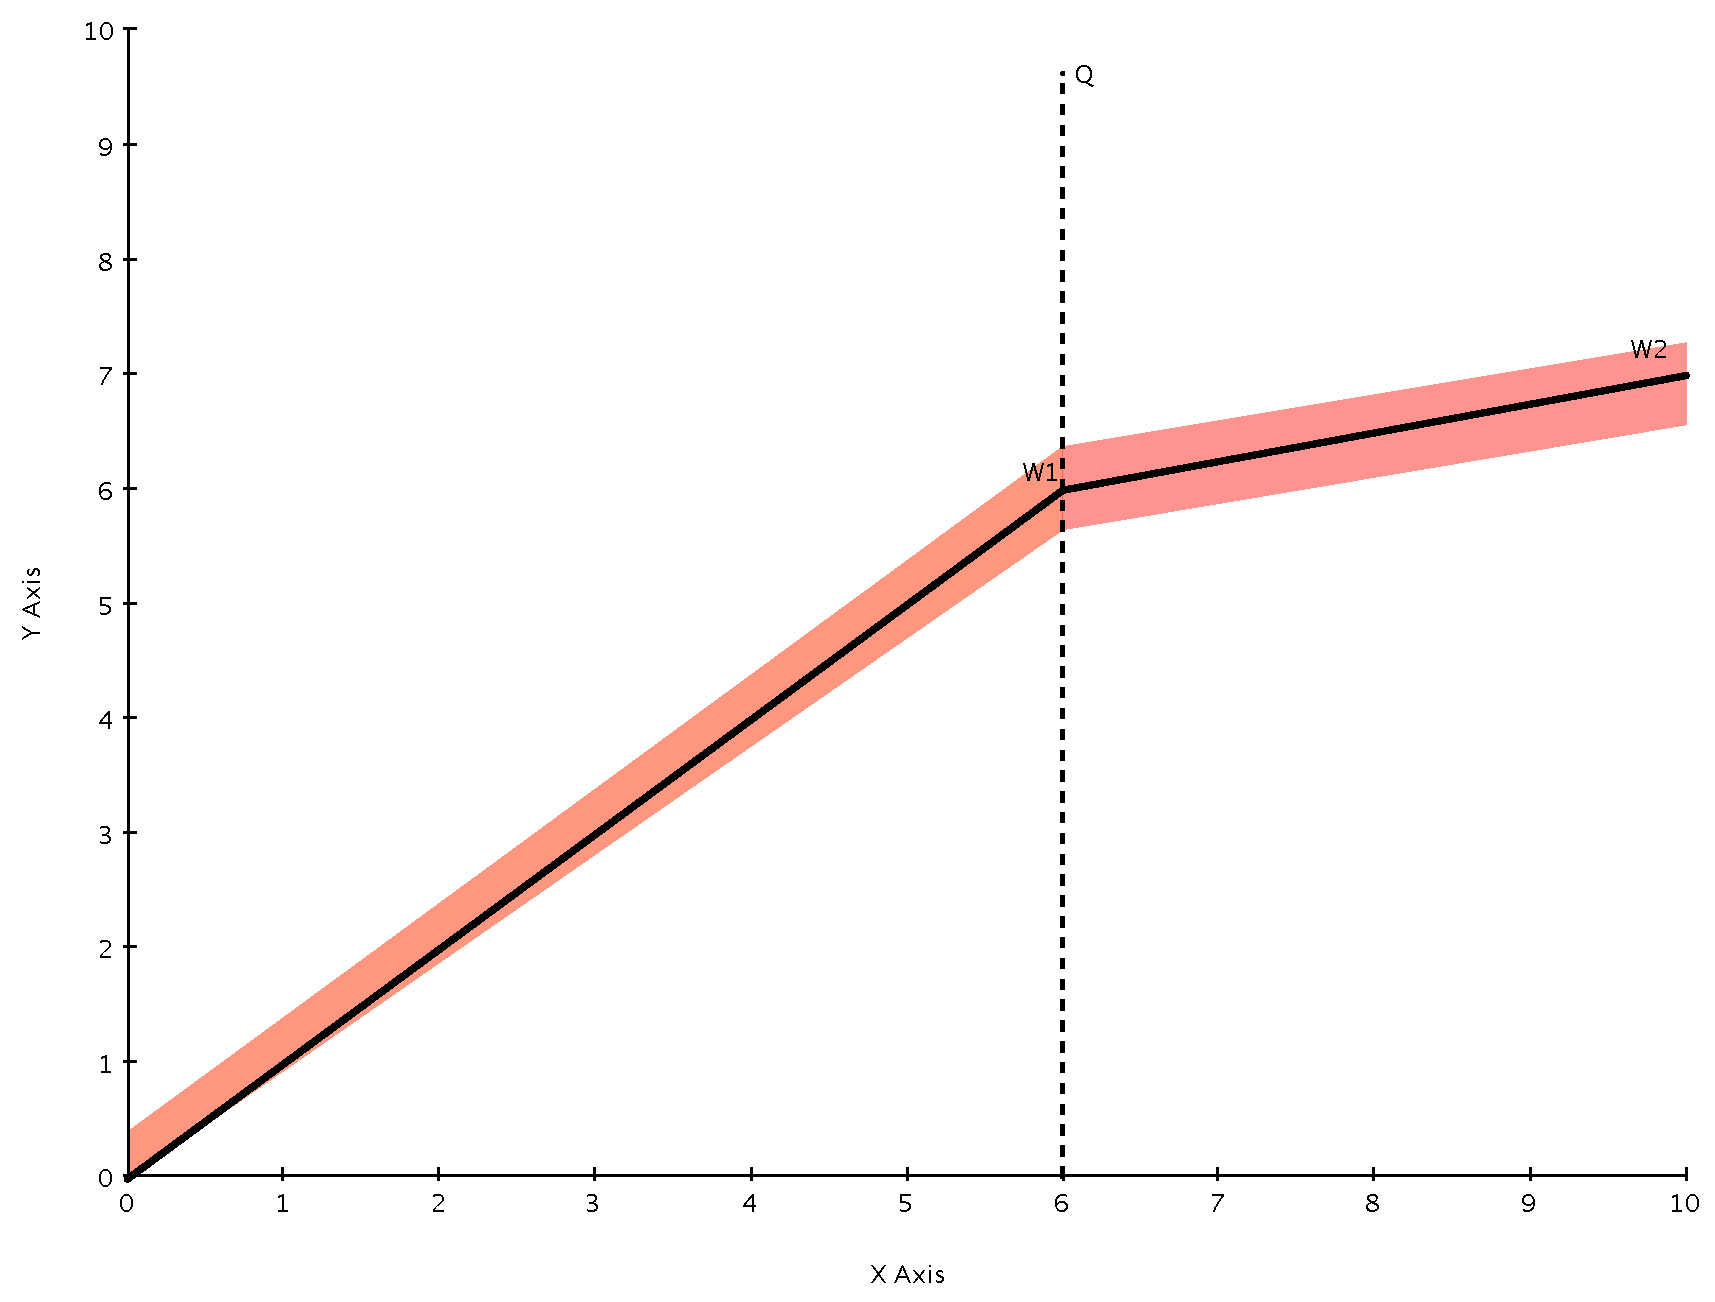
\includepdf[pages=1]{standardrebates.pdf}
Vertical Rebates (All-Units Discounts) apply a linear discount retroactively to previous sales: \\
\vspace{0.25in}
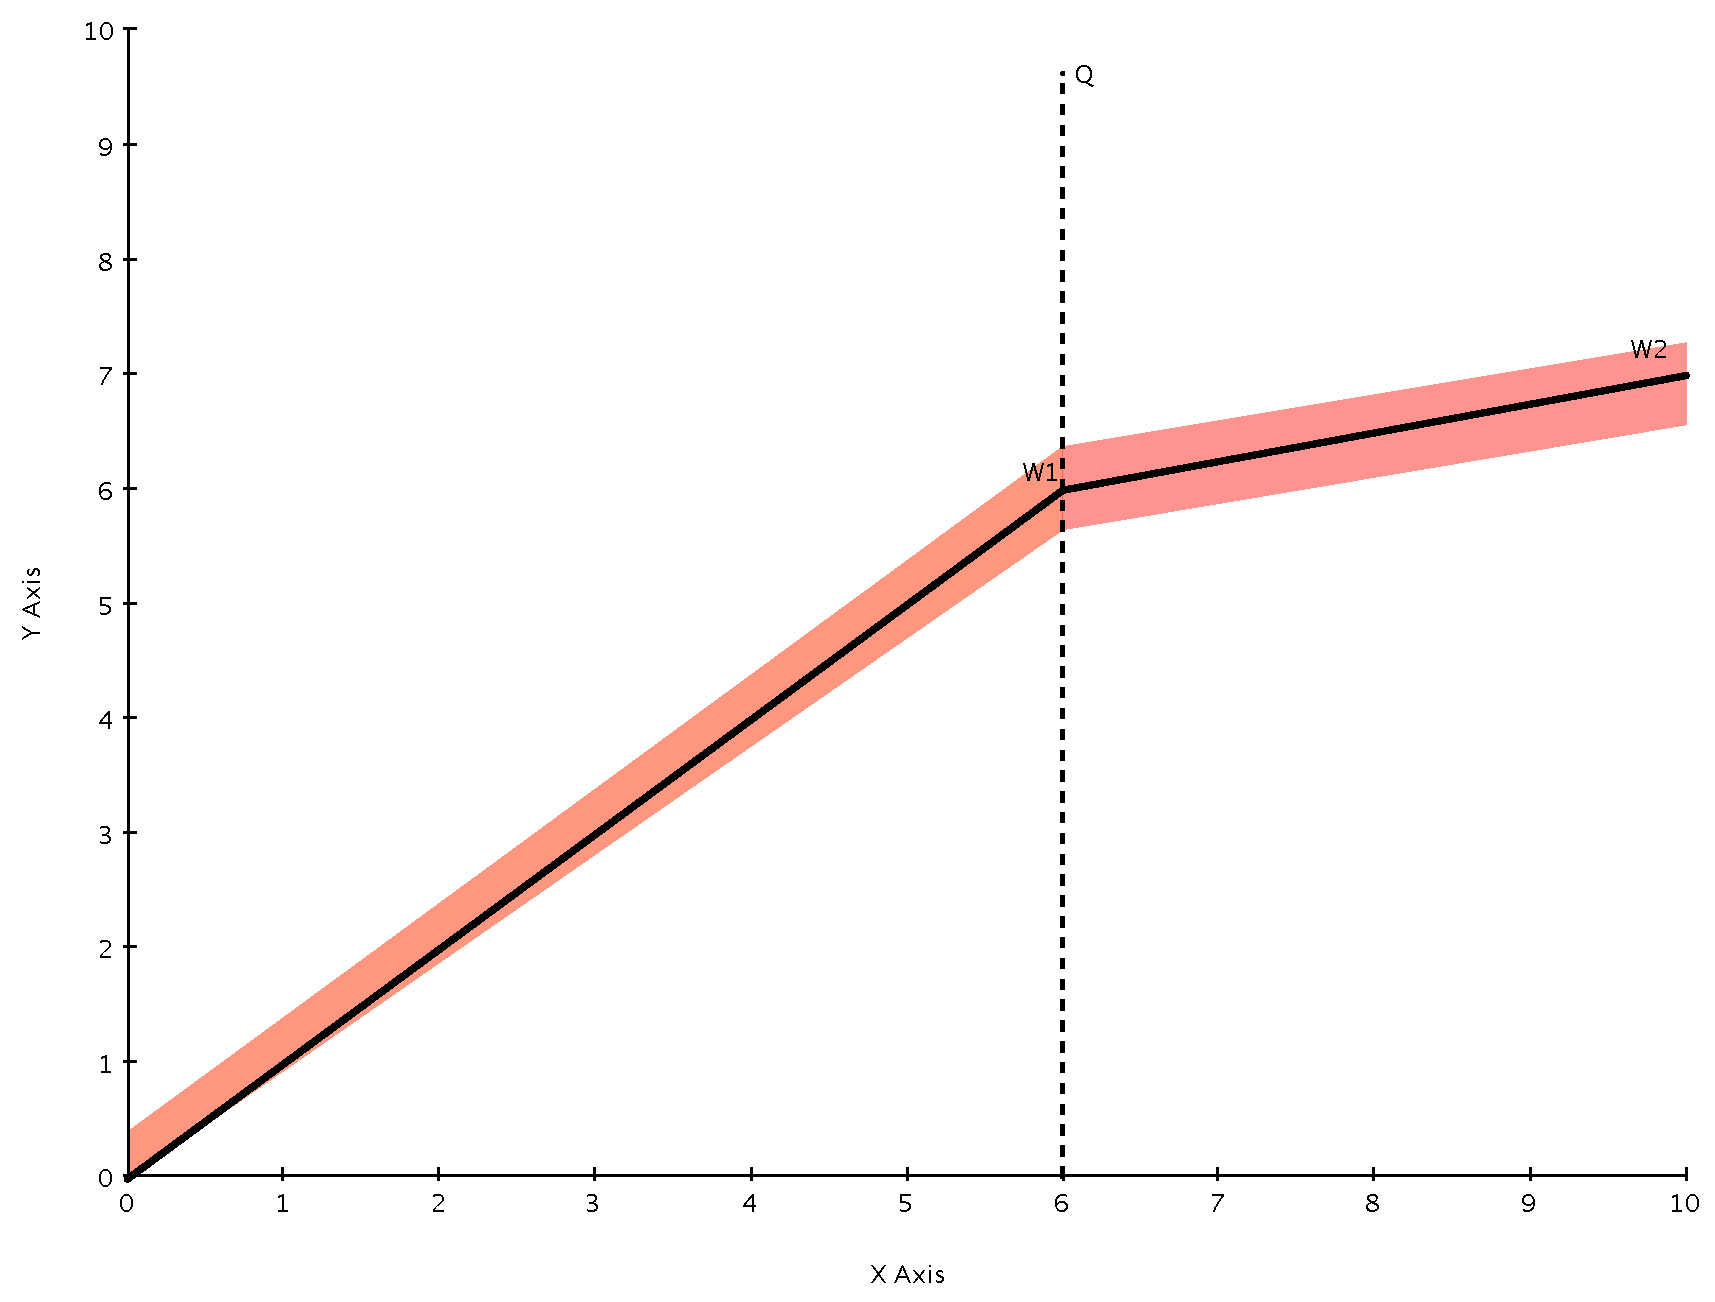
\includegraphics[width=.45\linewidth]{standardrebates.pdf} \hspace{0.25in} 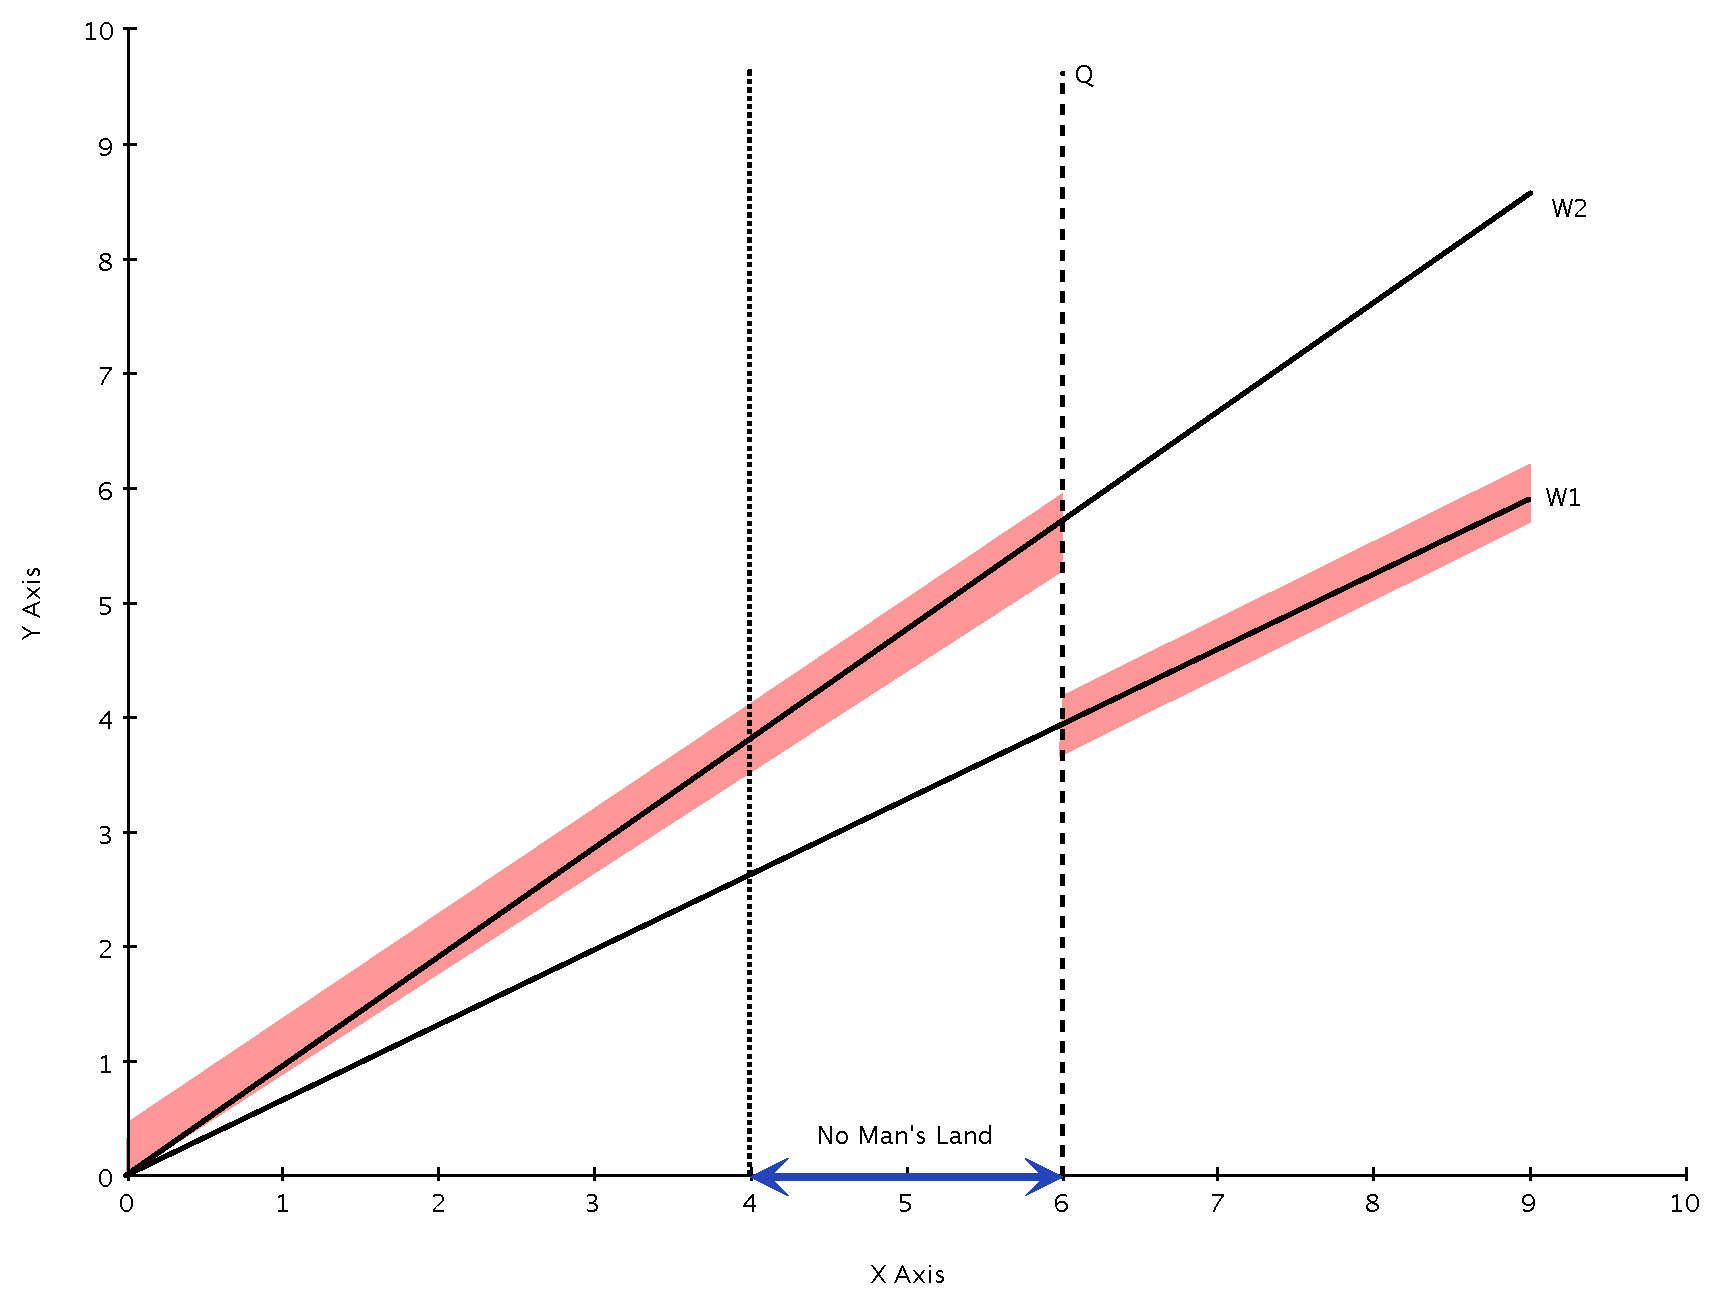
\includegraphics[width=.45\linewidth]{allunitsdiscount.pdf}
\begin{center}
\footnotesize
\hspace{-0.3in}Standard Non-linear Pricing \hspace{0.9in} All-Units Discounts
\end{center}
}


\begin{frame}
\frametitle{Efficiency vs. Foreclosure}
\small
At issue are the contracts' potential efficiency and foreclosure effects.\\
\vfill
Efficiency effects include:
\begin{itemize}\small
\item Aligning incentives of upstream and downstream firms
\item Incentivizing costly effort by downstream firms
\item Eliminating double marginalization or downstream moral hazard.
% (Telser 1960, Tirole).
\end{itemize} 
Foreclosure effects include:
\begin{itemize}\small
\item Reducing competition from other manufacturers
\item Reducing retail shelf-space or service levels on competitor's products
\item Substituting brands that compete closely with brands that don't.
\item Carrying underperforming brands by a rebating manufacturer.
\end{itemize} 
\end{frame}


\begin{frame}
\frametitle{Use of Vertical Rebates}
\begin{itemize}
%\item AUDs feature prominently in many vertically-separated industries (e.g., pharmaceuticals, hospital services, microprocessors, snack foods, heavy industry)
\item Used prominently in many vertically-separated industries 
\item A wide range of different settings:
	\begin{itemize}
	\item Used by dominant/competitive upstream firm? 
	\item Does it reference rivals? 
	\item Are multiple products covered? (If so, facing requirements?)
	\item Is there downstream price competition?
	\end{itemize}
\item A few recent anti-trust cases: 
	\begin{itemize} \footnotesize
	\item \textit{LePages v. 3M (2004)}: rebates on branded and private-label tape products found to be exclusionary.
	\item \textit{Cascade Health Solutions v. PeaceHealth (2008)} and \\ \textit{Eisai v. Sanofi-Aventis (2014)}: hospital care/pharmaceutical rebates alleged to be exclusionary, allowed (price-cost test) \\
	\item \textit{Intel (2009)}: Marketshare-based rebates, found by the European Comission to be anticompetitive. (\$1.4 billion fine.)
	\item \textit{Meritor v. Eaton (2012)}: rebates in heavy-duty truck transmission, found in violation of Sherman, Clayton Acts.
%	\item : rebates on a pharmaceutical product alleged to be exclusionary, but the courts allowed the rebates based on a price-cost test
	\end{itemize}
\end{itemize}
\end{frame}


\begin{frame}\frametitle{Challenges}
\begin{itemize}
\item Vertical rebates are widely used, the subject of frequent litigation; important to understand their effects.
\item Tension between efficiency and foreclosure effects requires empirical analysis to understand a contract's effects.
\begin{itemize}
\item Unfortunately, vertical contracts are considered proprietary by firms, frustrating many empirical studies
\item And, measuring downstream effort can be difficult
\end{itemize}
\item Our Approach:
\begin{itemize}
\item Examine an AUD contract using detailed data from one retailer
\item Conduct a field experiment in product stocking to identify: substitution patterns, and the relative cost of downstream moral hazard for upstream firms.
\item Estimate models of demand and retailer re-stocking to identify impacts of retailer decisions, and effects of AUD.
%\item Use exogenous variation (field experiment) for identification
%\item Identification makes use of a field experiment that directly manipulates the outcome of downstream effort (availability)
%, we find evidence of both efficiency and foreclosure effects of vertical rebate contracts.
\end{itemize}
\end{itemize}
\end{frame}

\begin{frame}
\frametitle{A Partial Literature Review}
\small
Theoretical Views on Vertical Contracts: Efficiency vs. Foreclosure
\footnotesize
\begin{itemize}
\item Chicago Critique: Bork (1978), Posner (1976)
\item Game-theoretic response: Aghion \& Bolton (1987), Bernheim \& Whinston (1998), Fumagalli \& Motta (2006)
\item Efficiency effects: Telser (1960), Klein \& Murphy (1988), Deneckere, Marvel \& Peck (1996, 1997)
\item Anti-competitive effects and exclusion: Shaffer (1991a/b), Rasmusen, Ramseyer \& Wiley (1991), Segal \& Whinston (2000), Inderst \& Shaffer (2010), Asker \& Bar-Isaac (2014)
\item All-Units Discounts: Kolay, Shaffer, \& Ordover (2004), O'Brien (2013), Chao \& Tan (2013)
\end{itemize}
\small
Empirical Work: Downstream Effort/Moral Hazard, Exclusive Contracts
\footnotesize
\begin{itemize}
\item Vertical Integration: Lafontaine (1992), Baker and Hubbard (2003), Crawford, Lee, Whinston and Yurukoglu (2015)
\item Exclusive contracts: Lee (2013), Sinkinson (2014)
\end{itemize}
\end{frame}


\frame{\frametitle{The Application and Research Question}
Vending Industry:
\begin{itemize}
\item \$41 billion, vertically-separated industry
\item Many small independent downstream operators 
\item No within-product (category) price variation
\item Focus on confections/candy (vending is about 1/3 of sales).
\item Concentrated upstream market (Mars, Hershey, Nestle).
\item The largest firm, Mars, Inc., offers an AUD.
\item Like most contracts, this one has never been litigated.
\end{itemize}
Research Question: 
\begin{itemize}
\item What are the efficiency and foreclosure effects of an All-Units Discount used by Mars, Inc. in the confections industry?
\end{itemize}

}


\begin{frame}\frametitle{Main Findings}
%\footnotesize
%Main Findings:
\begin{itemize}
\item Mars' AUD affects retailer assortment choice:
	\begin{itemize}
	\item Favors Mars' products over Hershey's, foreclosing Hershey.
	\item Consumers prefer `all Mars' to `all Hershey' assortment.
	\item But consumers' most-preferred assortment is a Mars/Hershey mix, which is not supported by the AUD.
	\end{itemize}
\item Mars' AUD also leads to increased retailer effort:
\begin{itemize}
\item Better service for Mars and consumers (faster re-stocking).
\item Hershey and Nestle lose (Mars products don't stock-out).
\item But efficiency effect alone cannot justify the contract.
%\item Foreclosure: Hershey is excluded; the contract fails to implement effort or assortment that is socially (or industry) optimal.
\end{itemize}
\item Observed contracts are close to optimal (given wholesale p)
%\item Welfare effects depend on what happens without an AUD.
%	\begin{itemize}
%	\item Hold wholesale prices fixed
	%\item Let Mars re-optimize its linear price
\item Upstream mergers may mitigate foreclosure incentives, but may also reduce retailer profit.
%	\end{itemize}
%are positive, compared to removing the AUD at current wholesale prices.
%	\begin{itemize}
%	\scriptsize
%	\item Merging with a close substitute may lower efficiency gains but eliminate the incentive to foreclose
%	\item Merging with a product that doesn't substitute may increase incentives to pay for efficiency but maintain incentives to foreclose other rivals
%	\end{itemize}
\end{itemize}
%	\begin{itemize}
%	\item Substitutability of products 
%	\item Substitutability of downstream effort
%	\end{itemize}
\end{frame}


\section{Data \& Experiment}
%\section{Effects of Product Removals}

\begin{frame}
\frametitle{Mars Rebate Program, 2010}
\begin{figure}
\begin{center}
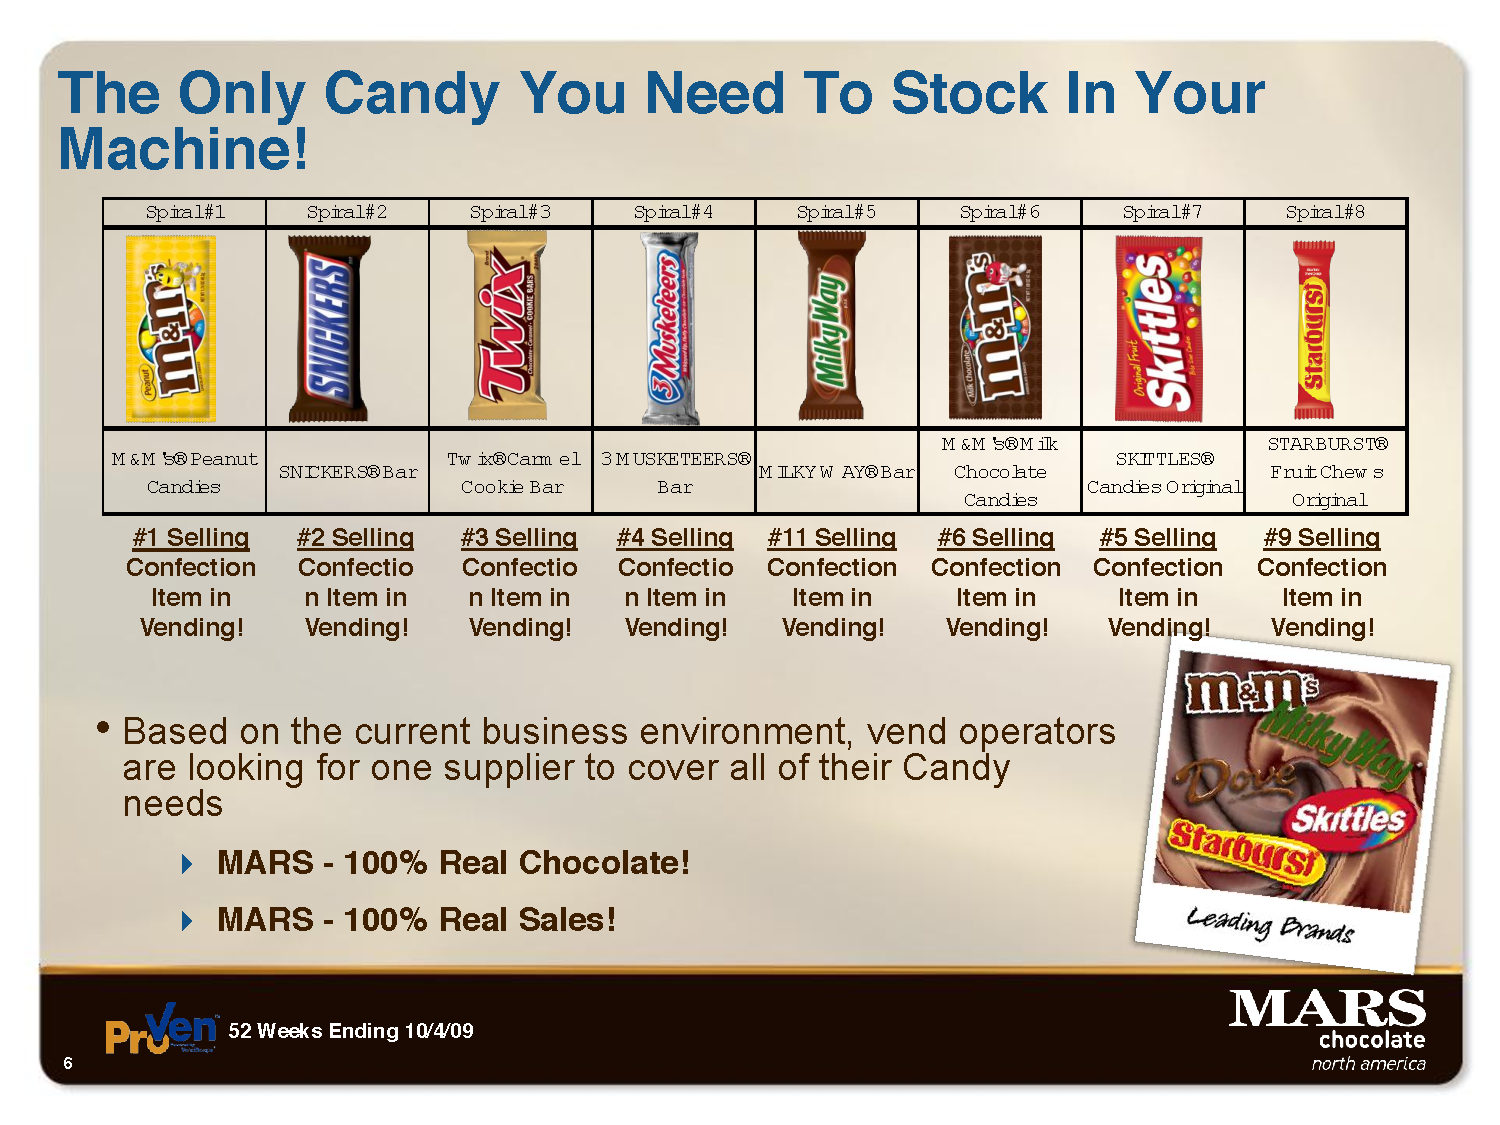
\includegraphics[width=.95\linewidth]{rebate1.pdf}\\
%\includegraphics[width=6in]{rebate2.pdf}
\label{fig:marsslides}
%\caption{Mars Vend Operator Rebate Program}
\end{center}
\end{figure}
\end{frame}

\begin{frame}
\frametitle{Mars Rebate Program, 2010}
\begin{figure}
\begin{center}
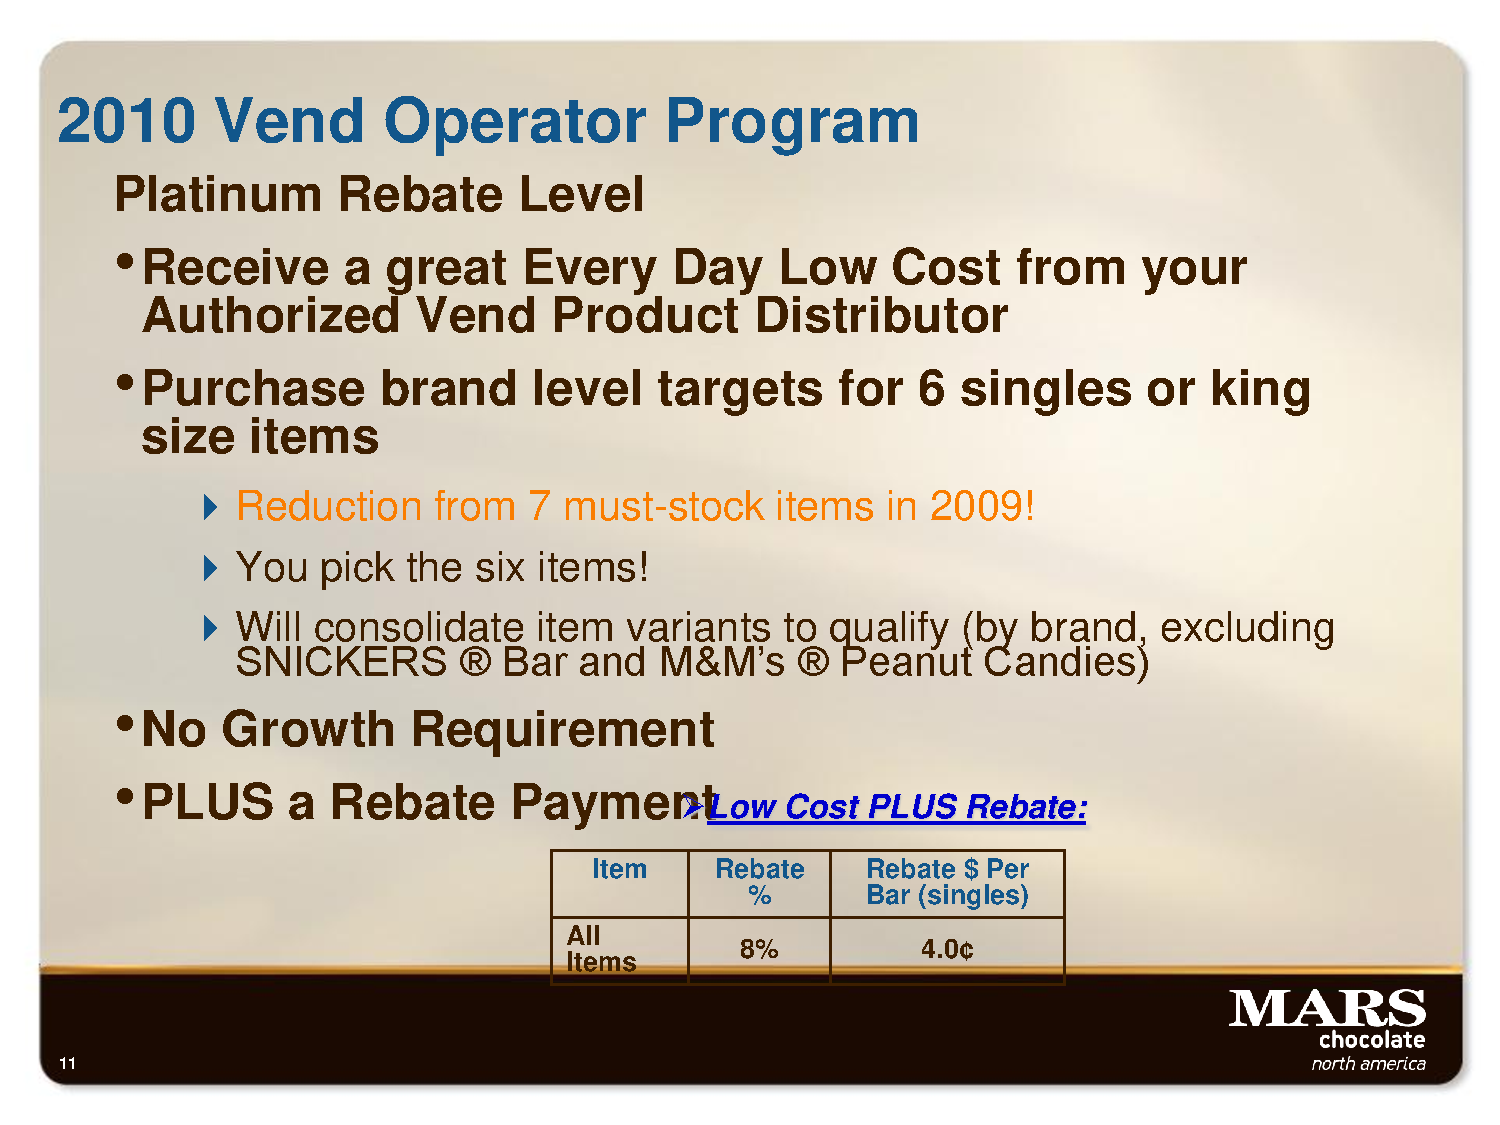
\includegraphics[width=.95\linewidth]{rebate3.pdf}\\
%\includegraphics[width=6in]{rebate2.pdf}
\label{fig:marsslides}
%\caption{Mars Vend Operator Rebate Program}
\end{center}
\end{figure}
\end{frame}


\frame{\frametitle{Data}
Detailed data from Mark Vend 
\begin{itemize}
\item A mid-sized vending operator in the Chicago area
\item Retail and wholesale prices, quantities, rebate payments.  
\item Enterprise-wide data, over a 38-month period: \\ January 2006 - February 2009.
\end{itemize}
}

\frame{\frametitle{Prices}
\begin{itemize}
\item At Mark Vend, retail prices are fixed at the category level. 
\item All confections are sold for 75 cents.
%\item We observe the wholesale prices that the retailer pays to each manufacturer.
\item We observe wholesale prices paid and terms of Mark Vend's AUD rebate program. We cannot disclose those directly.
\item Other manufacturers do not offer rebates (or `rebate' without a quantity threshold).
%\item Mars leaked a copy of very similar rebate terms in 2010.
\end{itemize}
}


\begin{frame}
\frametitle{Mark Vend's Assortment}
\begin{center}
\vspace{-0.3in}
\scriptsize
Comparison of National Availability and Shares with Mark Vend
\begin{tabular}{|l|l|c|r|r|r|r|}
\hline
&&\multicolumn{3}{c|}{National:}&\multicolumn{2}{c|}{Mark Vend:} \\
Manu-& &&Avail-&& Avail- &  \\
facturer&Product &Rank&ability&Share& ability & Share \\
\hline \hline 
Mars& Snickers &1&89&12.0&96&22.0\\
Mars& Peanut M\&M&2&88&10.7&96&23.0\\
Mars& Twix Bar&3&67 &7.7&79&13.0\\
Hershey& Reeses Peanut Butter Cups &4&72&5.5& 29&3.7\\
Mars& Three Musketeers &5&57&4.3& 34&4.3\\
Mars& Plain M\&M  &6&65&4.2& 47&6.4\\
Mars& Starburst &7&38&3.9& 16&1.0\\
Mars& Skittles &8&43&3.9& 77&6.5\\
Nestle& Butterfinger &9&52&3.2& 33&2.7 \\
Hershey & Hershey with Almond &10&39&3.0&  0&0\\
%11&47.2& Mars & Milky Way/Payday & 33 & 2.6\\
Nestle& Raisinets &$>$45 &N/R &N/R& 78& 8.9\\
\hline
\end{tabular}\\
\end{center}
\begin{spacing}{0}
\tiny Notes: National Rank, Availability and Share refers to total US sales for the 12 weeks ending May 14, 2000, reported by Management Science Associates, Inc., at http://www.allaboutvending.com/studies/study2.htm, accessed on June 18, 2014.  National figures not reported for Raisinets because they are outside of the 45 top-ranked products.  By manufacturer, the national shares of the top 45 products (from the same source) are: Mars 52.0\%, and Hershey 20.5\%.  For Mark Vend, shares are: Mars 80.0\%, Hershey 8.5\% (calculations by authors).  Mark Vend averages 6.86 confection facings per machine.
\end{spacing}
\end{frame}

\begin{frame}{Response to Threshold: Assortment}
\small
\begin{center}
\begin{tabular}{|l | rrr | rrr|} \toprule
 & & Total & Mars  & &  &  \\ 
Quarter &   Index \% & Vends & Share & Mars & Hershey & Nestle \\ \midrule
2007q1 & 109.16 & 1,000.00 & 20.20 & 6.61 & 1.13 & 1.58 \\
2007q2 & 106.29 & 1,087.45 & 19.77 & 6.24 & 1.44 & 1.17 \\
2007q3 & 100.81 & 1,008.57 & 20.94 & 6.21 & 1.63 & 1.08 \\
2007q4 & 105.23 & 1,092.49 & 19.97 & 6.26 & 1.73 & 1.03 \\ \midrule
2008q1 & 106.27 & 1,103.42 & 19.45 & 5.98 & 2.08 & 0.97 \\   \midrule
2008q2 & 97.20 & 1,057.32 & 19.77 & 5.57 & 2.29 & 0.93 \\ 
2008q3 & 91.88 & 1,014.13 & 19.14 & 5.37 & 2.29 & 0.91 \\
2008q4 & 87.02 & 1,048.26 & 18.11 & 5.48 & 2.19 & 0.89 \\
2009q1 & 87.03 & 1,058.54 & 17.65 & 5.32 & 1.99 & 0.83 \\ 
\bottomrule
\end{tabular}
\end{center}

Right three columns report facings per machine by manufacturer.
\end{frame}

\begin{frame}{Assortment Detail: Facings Per Machine}
\footnotesize
\begin{center}
\begin{tabular}{|c | r r r r|}\midrule
&\multicolumn{2}{c}{Mars products:}&\multicolumn{2}{c|}{Hershey products:}\\
Quarter &  Milkyway &  3 Musketeer & Reese's PB & Payday \\
\toprule
2006q1 & 0.26 & 0.50 & 0.19 & 0.08 \\
2006q2 & 0.26 & 0.49 & 0.15 & 0.03 \\
2006q3 & 0.29 & 0.56 & 0.03 & 0.01 \\
2006q4 & 0.31 & 0.55 & 0.01 & 0.04 \\
2007q1 & 0.32 & 0.56 & 0.00 & 0.08 \\
2007q2 & 0.31 & 0.53 & 0.00 & 0.18 \\
2007q3 & 0.29 & 0.54 & 0.01 & 0.21 \\
2007q4 & 0.30 & 0.51 & 0.15 & 0.20 \\ \midrule
2008q1 & 0.38 & 0.29 & 0.51 & 0.19 \\  \midrule
2008q2 & 0.43 & 0.03 & 0.66 & 0.21 \\ 
2008q3 & 0.41 & 0.00 & 0.63 & 0.23 \\
2008q4 & 0.40 & 0.01 & 0.62 & 0.24 \\
2009q1 & 0.37 & 0.01 & 0.62 & 0.23 \\ \bottomrule
\end{tabular}
\end{center}
\end{frame}


\begin{frame}{Response to Threshold: Effort}
\begin{table}
\caption{Effort Response to Changes in the Threshold}
\begin{center}
\label{tab:effort}
\begin{tabular}{|l|cc|} \hline
& Vends Per Visit & Elapsed Days Per Visit \\ \hline
 &  &  \\
Lower Threshold & 8.262*** & 0.857*** \\
 & (0.410) & (0.0690) \\
 &  &  \\
Observations & 117,428 & 117,428 \\
R-squared & 0.361 & 0.154 \\
Machine FE & YES & YES \\
 Week of Year FE & YES & YES \\ \hline
\multicolumn{3}{c}{ Standard errors in parentheses} \\
\multicolumn{3}{c}{ *** p$<$0.01, ** p$<$0.05, * p$<$0.1} \\
\end{tabular}
\end{center}
%\footnotesize Notes: 
\end{table}
\end{frame}

\frame{\frametitle{Exogenous Product Removals}
In addition to the detailed data on p, q, and rebate payments, Mark Vend ran a field experiment for us:
\begin{itemize}
\item Exogenously remove Snickers, Peanut M\&Ms, or both.
%, without any restocking response by the retailer.
\item Simulates impact of re-stocking effort; identifies substitution.
% on the upstream and downstream firms.
\end{itemize}
Experimental Setting:
\begin{itemize}
%\item Mark Vend, a mid-size vending operator
\item 66 snack machines in office buildings in downtown Chicago
\item For each run, remove product(s) for 2.5-3 weeks from all machines at each site.
%\item Machines are visited 3 times on avg.  during each removal.
%\item Data collected from January, 2006 - February, 2009.
\item Interventions run during May - October, 2007 and 2008.
\item For details, see our other papers.
\end{itemize}
}

\frame{\frametitle{Profit/Revenue Impacts of the Product Removals}
\small 
Downstream Profit
\scriptsize
\begin{table}
\begin{center}
\label{tab:nonparamprofit_total}
\begin{tabular}{|lrr|rrr|rrr|}
\hline
& & & \multicolumn{3}{c|}{Before Rebate} & \multicolumn{3}{c|}{After Rebate} \\
\hline
& & & \multicolumn{2}{c}{Difference In:}& T-Stat & \multicolumn{2}{c}{Difference In:} & T-Stat \\
Removal & Vends & &  Margin & Profit & of Diff & Margin & Profit & of Diff \\
\hline \hline
Snickers &-216.82&&0.39&-56.75&-2.87&0.24&-73.26&-4.33\\
Peanut M\&Ms&-197.58&&0.78&-10.74&-0.58&0.51&-39.37&-2.48\\
Joint&-282.66&&1.67&-4.54&-0.27&1.01&-54.87&-3.72\\
\hline\end{tabular}
\end{center}
\scriptsize
% obs: 109 (snickers) 115 (peanut mm) 89 (joint)
%Notes: Rebates is direct transfer from Mars to Retailer.
Note: Rebate is a direct transfer from Mars to Retailer.\\
\end{table}
\vfill
\small 
Upstream Revenue
\scriptsize
\begin{table}
\begin{center}
\begin{tabular}{|l|rrrr|rr|}
\hline
 &\multicolumn{4}{c|}{Pre-Rebate Impact of Removal on:}& \multicolumn{2}{c|}{Cost Born by Mars} \\
Removal& Mars & Hershey &  Nestle & Other & \% Before & \% After \\
\hline \hline
Snickers&-26.37&5.89&19.32&-20.26&31.7\%&11.9\%\\
Peanut M\&Ms&-68.38&32.76&11.78&-9.36&86.4\%&50.2\%\\
Joint&-130.81&61.43&20.22&37.10&96.7\%&59.5\%\\
\hline\end{tabular}
\end{center}
Note: Revenues to manufacturer are calculated as the wholesale cost \\ paid by Mark Vend to the manufacturer.
\end{table}
%, not including any potential rebate payments.  
}



\section{Theory}

\begin{frame}[label=intuition]
\frametitle{Theory: Choice of Assortment}
%\begin{itemize}
%\end{itemize}
%\end{frame}
%\begin{frame}
%\frametitle{Theory: All Units Discounts}
Set-up, holding retail prices and effort fixed:
\begin{itemize}
\item Retailer $R$ has two marginal slots to fill.
\item Two producers, $M$ and $H$, selling two products each.
%\item Retail prices are fixed.
\item Retailer can choose three assortments: $a \in \{ (H,H), (H,M), (M,M)\}$.
%\item In absence of rebate, can order the profits for each agent:\\
%R, H prefer $(H,H) > (H,M) > (M,M)$\\
%M prefers $(H,H) < (H,M) < (M,M)$\\
\end{itemize}
\end{frame}



\begin{frame}
\frametitle{Theory: Foreclosure with All Units Discounts}
\begin{itemize}
\item Suppose $M$ offers an AUD:
	\begin{itemize}
	\item If: $R$ sells at least $\overline{q}_m$ units of $M$'s products 
	\item Then: $R$ receives a discount $d$ on all units.
	\end{itemize}
\item For constant marginal cost $c_M$ and linear wholesale price $w_M$, the discount is a fraction $\lambda$ of $M$'s profit.
%%\item AUD may induce full foreclosure that does not maximize industry profits.
%\item Without AUD, suppose $R$ chooses $(H,H)$ or $(H,M)$
%	\begin{itemize}
	\item If gains to $M$ of foreclosing $H$ exceed $H$'s gains, foreclosure is equilibrium outcome. ``Efficient'' by Chicago Critique.
	\item If $H$'s gains exceed gains to $M$, $M$ can still foreclose by requiring a higher threshold $\overline{q}_m$. Foreclosure via `tying' -- internalize demand externalities between products.
	\begin{itemize}
	\item Bernheim and Whinston's incentive conflict mechanism: bilateral payoffs are maximized, although industry profits fall.
	\end{itemize}
%	\item In both cases, $M$ can fully foreclose $H$. Foreclosure is ``efficient'' in first; ``inefficient'' in second (Chicago Critique).
%	\end{itemize}
\end{itemize}
\hyperlink{supplemental}{\beamerbutton{Additional Detail.}}
\end{frame}

%\begin{frame}
%\frametitle{Theory: Foreclosure with All Units Discounts}
%Result:
%\begin{itemize}
%\item AUD can be used to foreclose a rival (whether or not it maximizes industry profits).
%\item $M$ just needs to choose threshold $\overline{\pi}^M$ appropriately:\\ 
%%$\pi^M(H,H) < \pi^M(H,M) <  \pi^M(M,M)$
%%\item $\lambda \pi^M$ gives us access to a wide range of transfers for $\lambda \in [0,1]$.
%\begin{eqnarray*}
%\begin{cases}
% \pi^R(a) + \lambda \cdot \pi^M(a) &\mbox{ if } \pi^M(a) \geq \overline{\pi^M}\\
% \pi^R(a)     &\mbox{ if } \pi^M(a) < \overline{\pi^M}
%\end{cases}
%\end{eqnarray*}
%\item Ala Bernheim and Whinston (1998) with tying: achieve foreclosure, maximize bilateral payoffs of $M$ and $R$.
%\end{itemize}
%\end{frame}

\begin{frame}
\frametitle{Theory: Efficiency}
\begin{itemize}
\item AUD contract also has potential efficiency benefits
\item Suppose $R$ must exert costly effort $c(e)$ to sell the good.
\begin{itemize}
\item restocking (or, service, test-drives, lower retail price, etc.)
\end{itemize}
\item Holding fixed the assortment choice $a$
\begin{eqnarray*}
\label{effortchoice}
\begin{cases}
 \pi^R(e) -c(e) + \lambda \cdot \pi^M(e) &\mbox{ if } \pi^M(e) \geq \overline{\pi^M}\\
 \pi^R(e)  -c(e)   &\mbox{ if } \pi^M(e) < \overline{\pi^M}
\end{cases}
\end{eqnarray*}
\item $\pi^M(e)$ is increasing in effort
\item Both features of the contract can induce greater effort: 
\begin{itemize}
\item larger $\lambda$ makes $R$ consider the profits of $M$
\item larger choice of threshold $\overline{\pi^M}$ increases effort
\end{itemize}
%\item We quantify both channels in our application.
\end{itemize}
\end{frame}


\begin{frame}
\frametitle{Theory: Solving For Effort}
\begin{eqnarray*}
\label{effortchoice}
\begin{cases}
 \pi^R(e) -c(e) + \lambda \cdot \pi^M(e) &\mbox{ if } \pi^M(e) \geq \overline{\pi^M}\\
 \pi^R(e)  -c(e)   &\mbox{ if } \pi^M(e) < \overline{\pi^M}
\end{cases}\\
\end{eqnarray*}
Retailer choice of effort has three potential solutions:
\begin{enumerate}
\item Interior Solution to top eq. (with rebate): $e^{R}$
\item Constraint binds (with rebate):  $e$: $\pi^M(e) = \overline{\pi}^M$
\item Interior Solution to bottom eq. (no rebate): $e^{NR}$
\end{enumerate}
%We calculate these in our empirical exercise.
We can characterize other solutions to the effort problem:
\begin{itemize}
\item $e^{VI}$ maximizes bilateral surplus between $R$ and $M$
\item $e^{SOC}$ maximizes social surplus (including consumers).
\end{itemize}
\end{frame}

%\begin{frame}
%\frametitle{Theory: Solving For Effort}
%\begin{itemize}
%\item We can characterize other solutions to the effort problem:
%\begin{itemize}
%\item $e^{VI}$ maximizes bilateral surplus between $R$ and $M$
%\item $e^{SOC}$ maximizes social surplus (including consumers).
%\end{itemize}
%\end{itemize}
%\begin{eqnarray*}
%\footnotesize
% e^{NR} &=& \arg \max_e \pi^R(e) - c(e)\\
% e^{R} &=& \arg \max_e \pi^R(e)  - c(e) + \lambda \cdot \pi^M(e)\\
% e^{VI} &=& \arg \max_e \pi^R(e)  - c(e) + \pi^M(e)\\
% e^{IND} &=& \arg \max_e \pi^R(e)  - c(e) +   \pi^M(e) + \pi^H(e)\\
% e^{SOC} &=& \arg \max_e \pi^R(e)  - c(e) +   \pi^M(e) + \pi^H(e) + \pi^C(e)
%\end{eqnarray*}
%\end{frame}


\begin{frame}
\frametitle{Theory: Putting it together}
\small
%\begin{itemize}
%\item 
Retailer observes rebate $\lambda$, threshold $\overline{\pi}^M$ and chooses $(a,e)$.
%, assuming no uncertainty about payoffs. \\
\vfill
%\item Assume no uncertainty about payoffs.
%\end{itemize}
%\begin{eqnarray*}
%\footnotesize
%\max_{a,e} \begin{cases}
% \pi^R(a,e) -c(e) + \lambda \cdot \pi^M(a,e) &\mbox{ if } \pi^M(a,e) \geq \overline{\pi^M}\\
% \pi^R(a,e)  -c(e)   &\mbox{ if } \pi^M(a,e) < \overline{\pi^M}
%\end{cases}
%\end{eqnarray*}
Empirical questions:
\begin{itemize}
\item How does $M$ choose $(\lambda,\overline{\pi}^M)$?
\item Is $H$ foreclosed? Does foreclosure maximize industry profits? Could $H$ give up all profit to avoid foreclosure?
\item Are gains to effort sufficient to overcome potential losses from foreclosure?
\end{itemize}
Components of Empirical Model:
\begin{itemize}
\item Consumer Choice Model (Discrete-choice demand, without price.)
\item Model of Retailer Effort (Single-agent dynamic model of restocking.)
\end{itemize}
\end{frame}



\section{Estimation/Simulation}

\frame[label=param_main]
{\frametitle{Consumer Choice}
\footnotesize
Discrete Choice Random Utility Maximization:

\begin{eqnarray}
u_{ijt} = \delta_{jt} + \mu_{ijt} +\varepsilon_{ijt}.
\end{eqnarray}
$\delta_{jt} = d_j + \xi_t$ captures mean utility for product $j$ in market $t$: \\ includes 73 product, and 15,256 market (machine-visit) fixed effects
\vfill
%
%Nested Logit:
%\vfill
%Let ($\mu_{ijt} + \varepsilon_{ijt}) \sim$ GEV.  Choice probabilities are:
%\begin{eqnarray}
%p_{jt}(\delta, \lambda,a_t) &=& \frac{e^{\delta_{jt}/\lambda_l}( \sum_{k \in g_l \cap a_t} e^{\delta_{kt} /\lambda_l})^{\lambda_l-1}}{\sum_{\forall l } ( \sum_{k \in g_l \cap a_t} e^{\delta_{kt}/\lambda_l})^{\lambda_{l}} }
%\end{eqnarray}
%$\lambda_l$ governs within-group correlation, and $a_t$ is assortment stocked in $t$.\\
%Group by five product categories:
%\begin{itemize}
%\item chocolate candy, non-chocolate candy, cookie, salty snack, other
%\end{itemize}
%}

%\frame
%{\frametitle{Consumer Choice, cont.}
%\footnotesize

Random Coefficients:\\
\vfill
Let $\mu_{ijt} \sim f(\mu_{ijt} | \theta)$, where $\mu_{ijt} = \sum_l \sigma_l \nu_{ilt} x_{jl}$ where $\nu_{ilt} \sim N(0,1)$.  \\ Choice probabilities are:
%and $\sigma_l$ represents the standard deviation of the heterogeneous taste for product characteristic $x_{jl}$. The resulting choice probabilities are a mixture over the logit choice probabilities for many different values of $\mu_{ijt}$, shown here:
\vfill
\begin{eqnarray}
p_{jt} (\delta,\theta,a_t)= \int \frac{e^{\delta_{jt} +  \sum_l \sigma_l \nu_{ilt} x_{jl} }}{1+ \sum_{k \in a_t} e^{\delta_{kt} + \sum_l \sigma_l \nu_{ilt} x_{kl}}} f(v_{ilt} | \theta)
\end{eqnarray}\\
\vfill
Three continuous product characteristics:
\begin{itemize}
\item salt, sugar, and nut content
\end{itemize}
\hyperlink{param_supp}{\beamerbutton{Estimates}}
}




\begin{frame}
\frametitle{Supply Side}
Overview:
\begin{itemize}
\item Three manufacturers:  (M)ars, (H)ershey, (N)estle. \\ Only Mars offers an AUD.
\item Take manufacturer terms as given: $w_M, w_H, w_N, \lambda, \overline{\pi_M}$
\item Model retailer choice of assortment, $a$, and effort, $e$.%, at the existing contract terms.
%\item For insight into the effect of the AUD, resolve at different values of $\overline{\pi^M}$, etc.
\end{itemize}
Retailer Choice of Assortment:
\begin{itemize}
\item Assortment choice is discrete over a small number of alternatives. Compute it directly.
\end{itemize}
\end{frame}

\begin{frame}
\frametitle{Supply Side, cont.}

Retailer Choice of Effort:
\begin{itemize}
\item Mark Vend chooses an enterprise-level restocking policy at the beginning of each quarter.
	\begin{itemize}
	\item Translates the effort policy to a restocking schedule for each machine using machine-specific arrival rates.
	\item Once set, the schedule is broken into driver routes.
	\item In order to reduce the number of consumers between visits, Mark Vend requires additional routes, which increases his cost.
	\end{itemize}
\item Retailer chooses restocking frequency: Rust, but `in reverse.'
\begin{itemize}
\item Use data on cost of restocking; compute the optimal wait time.
\end{itemize}
\item Motivated by earlier evidence that re-stocking effort varies with threshold, but schedules are fixed within a quarter.
\end{itemize}
\end{frame}

\begin{frame}
\frametitle{Dynamic Model of Re-stocking}
\begin{itemize}
\item The retailer's value function is:
\begin{eqnarray}
\label{bellman}
V(x) = \max \{u(x) - FC + \beta V(0), \beta E_{x'}[V(x' | x)]\}
\end{eqnarray}
where $x$ is the number of potential consumers (a scalar).
\item Given a policy, compute post-decision transition-probability-matrix $\tilde{P}$ and utility $\tilde{u}$ given by:
\begin{eqnarray*}
 \tilde{u}(x,x^{*})= \begin{cases} 0 &\mbox{if } x < x^{*} \\ 
u(x) - FC & \mbox{if } x \geq x^{*}
 \end{cases}
\end{eqnarray*}
\item which solves the value function at all states in a single step:
\begin{eqnarray}
\label{pistep}
V(x,x^{*}) = (I - \beta \tilde{P}(x^{*}))^{-1} \tilde{u}(x,x^{*}) 
\end{eqnarray}
\end{itemize}
\end{frame}


\begin{frame}
\frametitle{Dynamic Restocking Procedure}
\small
\begin{itemize}
\item Of interest: a stationary long-run policy, $e \equiv x^{*}$ and $V(x,x^{*}).$
\item We can evaluate the pay-off of $R$, $M$, $H$, $N$, or any combination ($VI$, $IND$, $SOC$) given a fixed policy, $x.^*$
\item Equivalent to ``pre-committing'' to effort level before realizing sales, or setting an ``average service level.'' 
\item No demand uncertainty, many machines, so we can focus on the ergodic distribution of profits. (Makes the game static).
\end{itemize}
\end{frame}




\begin{frame}
\frametitle{Dynamic Restocking Procedure, cont.}
Given demand parameters $\hat{\theta}$:
\begin{enumerate}
\item Forward simulate sales for a machine with choice set $a$, from full to completely empty, as a function of $x$.
\item Choose an effort policy $e = x.^{*}$
\item Given $(w_H, w_N,w_M,\lambda,\overline{\pi^M})$, compute pay-offs for all agents.
\end{enumerate}
%\pause 
Details:
\begin{itemize}
\item Use a fixed cost of re-stocking of \$10. 
	\begin{itemize}
	\item Approximates the per-machine restocking cost using driver's wage and average number of machines serviced per day.
	\item Robust to reasonable alternative estimates.
	\end{itemize}
%\item Report results for three assortments that are relevant: $(H,H), (H,M)$, and $(M,M)$.
%\begin{itemize}
%\item $(H,H)$: Reese's PB Cup, Payday
%\item $(H,M)$: Reese's PB Cup, Three Musketeers
%\item $(M,M)$: Three Musketeers, MilkyWay
%\end{itemize}
\end{itemize}
\end{frame}

\begin{frame}[label=main]
\frametitle{Assortment Choice}
\begin{itemize}
\item Vending machines allow 7 confections products. Restrict attention to assortments that are not dominated.
\item Non-dominated assortments include five base products:
\begin{itemize}
\item Four Mars: Snickers, Peanut M\&M, Plain M\&M, and Twix. 
\item One Nestle: Raisinets.
\end{itemize}
\item Simulate results for 15 assortments: 5 base products and $6 \choose 2$ options for the final two slots.
%\begin{itemize}
%\scriptsize
%\item Two Mars products (Milkyway and 3 Musketeers)
%\item Two Hershey products (Reese's Peanut Butter Cup and PayDay)
%\item Two Nestle products (Butterfinger and Crunch).
%\end{itemize}
\item Provide results for three assortments that are relevant: $(H,H), (H,M)$, and $(M,M)$.
\begin{itemize}
\item $(H,H)$: Reese's PB Cup, Payday
\item $(H,M)$: Reese's PB Cup, Three Musketeers
\item $(M,M)$: Three Musketeers, MilkyWay
\end{itemize}
\end{itemize}
\hyperlink{supplemental1}{\beamerbutton{Details(1)}}
\hyperlink{supplemental2}{\beamerbutton{Details(2)}}
\end{frame}


\section{Results}

\begin{frame}
\frametitle{Assortment Decisions with Effort Policy $e^R$}
Holding effort fixed, look at assortment decision
\begin{table}[htp]
\caption{Agent Profits}
\begin{center}
\begin{tabular}{|l| rrr|}
\hline
 & (H,H) & (H,M) & (M,M) \\
 \hline
$e^{R}$ & 257 & 261 & 259 \\ \hline
$\pi^R$ & 36,656 & 36,394 & 36,086 \\
$\lambda \pi^M$ & 1,617 & 1,882  & 2,096\\
$\pi^M$ & 10,106 & 11,763 & 13,101 \\
$\pi^H$ & 2,167 & 1,299 & 0 \\
$\pi^{R} +\pi^{M}$ & 46,762 & 48,157 & 49,187 \\
$\pi^R + \pi^M + \pi^H$ & 48,929 & 49,456 & 49,187 \\ \hline
\end{tabular}
\end{center}
\label{tab:assortmentonly}
\end{table}
\end{frame}

\begin{frame}
\frametitle{Assortment Decisions with Effort Policy $e^R$, cont.}
\vspace{-0.4in}
\begin{table}[htp]
\caption{Changes in Profit}
\begin{center}
\begin{tabular}{|l| rrr|}
\hline
from &\hspace{0.15in} $(H,H)$ &\hspace{0.15in} $(H,M)$ & \hspace{0.15in}$(H,H)$ \\
to &\hspace{0.15in} $(H,M)$ & \hspace{0.15in}$(M,M)$ & \hspace{0.15in}$(M,M)$\\
 \hline
$\Delta \pi^R$&   -262 & -308& -570 \\
$\Delta \pi^M$ &  1,657 & 1,338 & 2,995 \\
$\Delta \pi^{M+R}$&   1,395 & 1,030& 2,425 \\
$\Delta \pi^H$  &-868 & -1,299 & -2,167 \\
 \hline
 \end{tabular}
\end{center}
\label{tab:assortmentonly2}
\end{table}
\vspace{-0.3in}
\begin{table}[htp]
\begin{center}
%Rebates\\
%\vspace{0.02in}
\caption{Changes in Producer and Consumer Surplus}
\begin{tabular}{|l| rrr|}
\hline
% &\multicolumn{3}{c|}{Rebates}\\
Feasible & 262-1,657 & 308-1,338&570-2,995 \\
Observed & 1,882 & 214& 2,096 \\
\hline
$\Delta PS$ & 501 & -272 & 229 \\
$\Delta CS$ &261 & -110 & 150 \\
$\Delta SS$ &762 & -383 & 379 \\ \hline
\end{tabular}
\end{center}
\label{tab:assortmentonly3}
\end{table}

\end{frame}

\begin{frame}
\frametitle{Impact of AUD Quantity Threshold on Retail Assortment}

 \begin{figure}[h!]
\begin{center}
%\caption{Impact of AUD Quantity Threshold on Retail Assortment Choice}
\vspace{-0.1in}
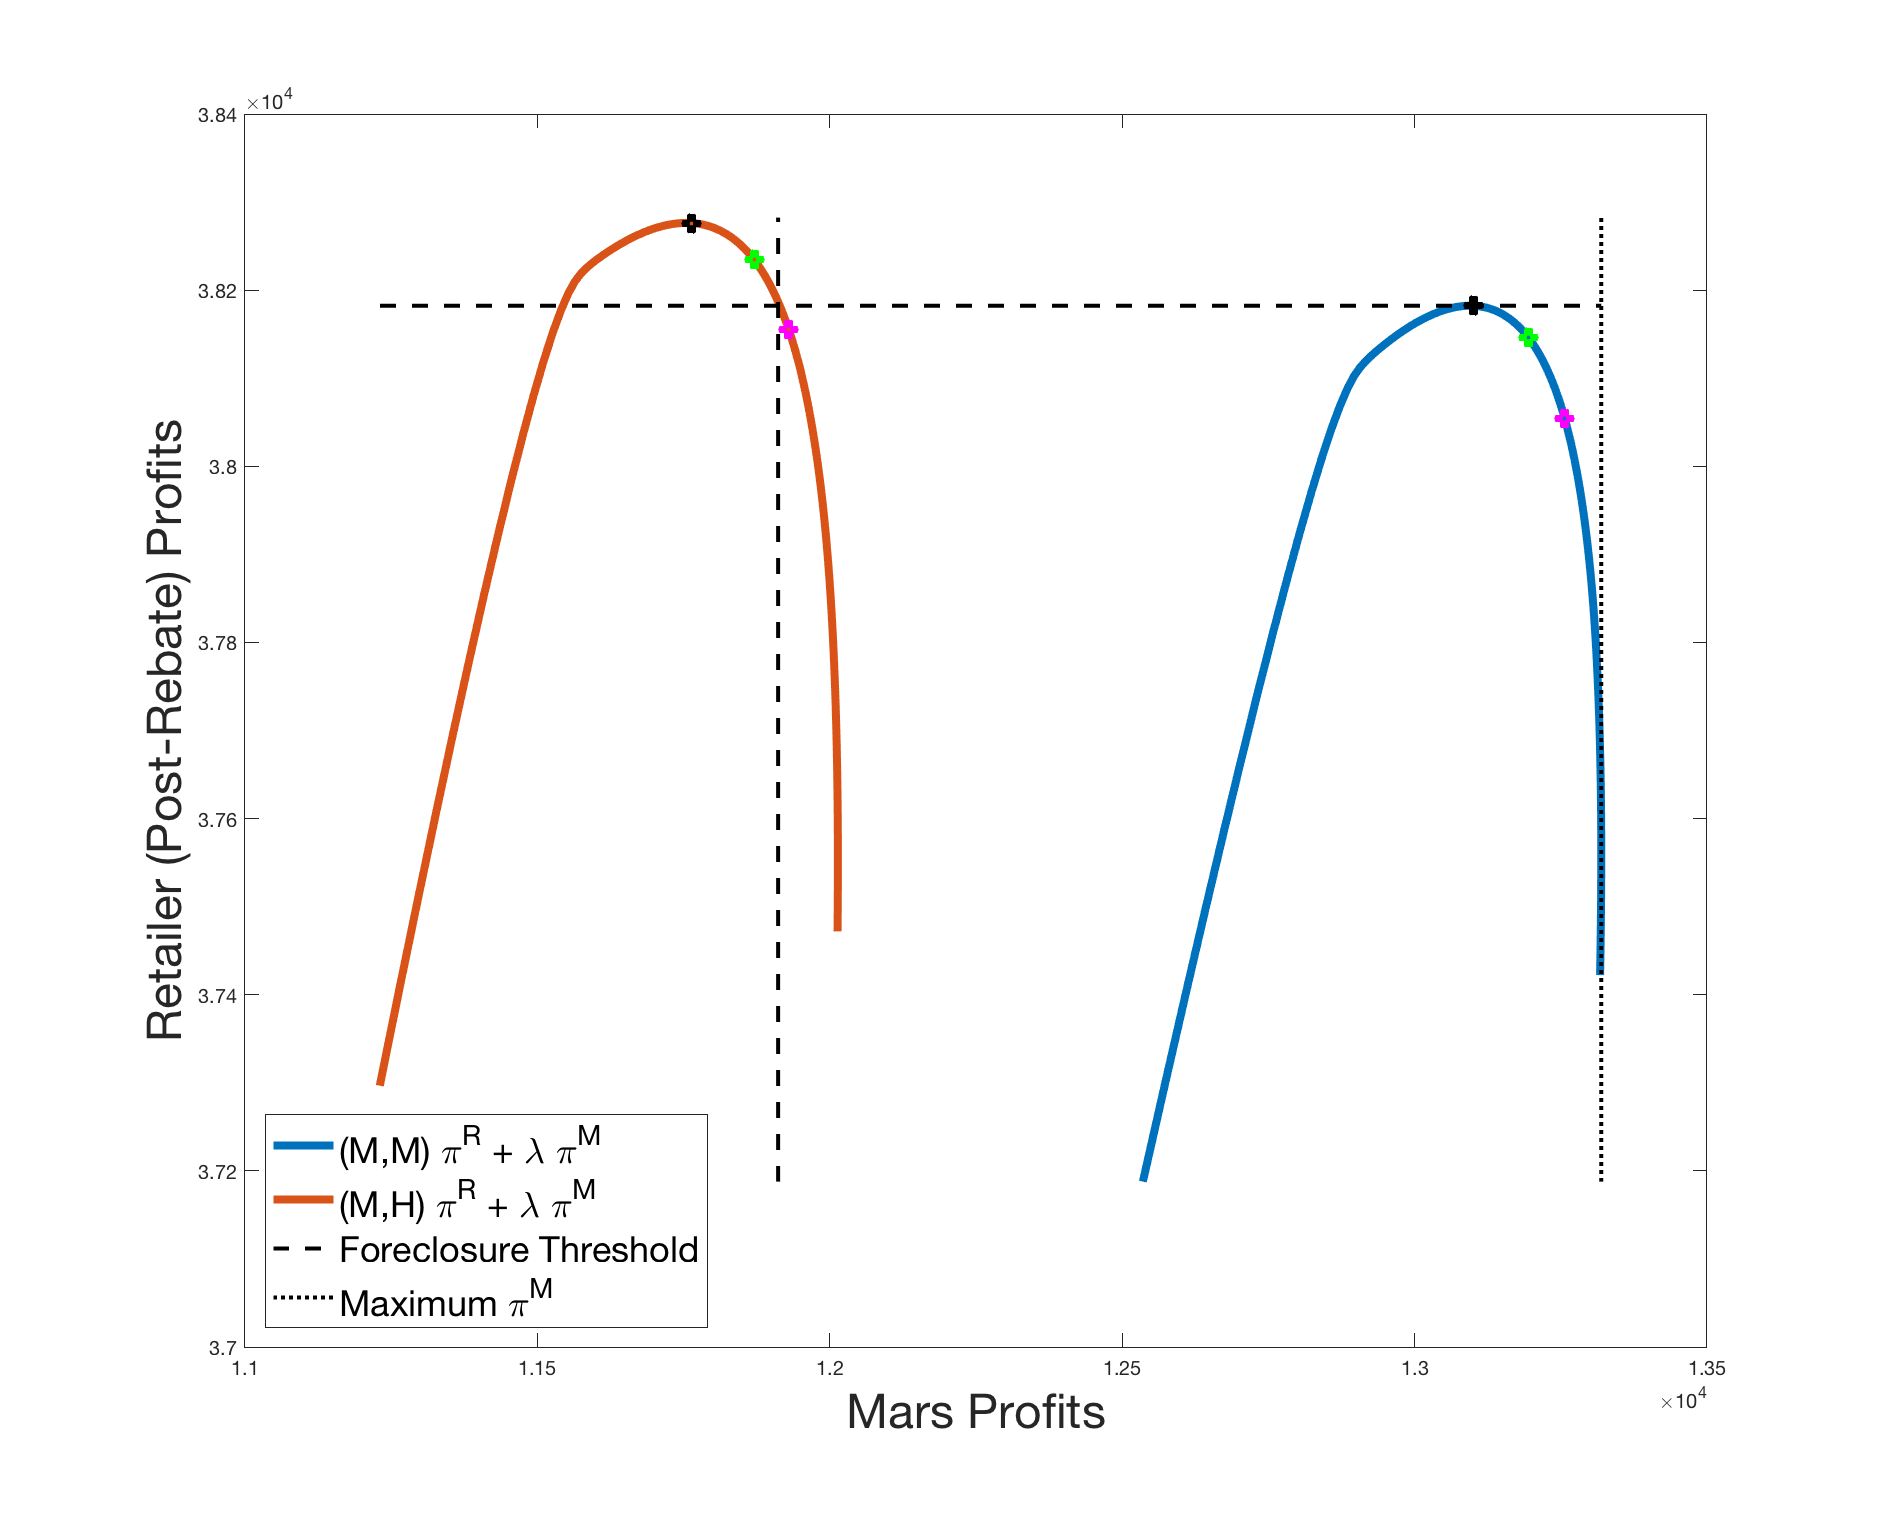
\includegraphics[width=3.4in]{newfigure4.png}
\label{fig:threshold}
\end{center}
\tiny
Notes: Figure reports retailer profit under two assortment choices ((H,M) on the left and (M,M) on the right), against sales of Mars products.  For a threshold $\overline{\pi}^M \geq 11,912$ (noted by the vertical dashed line), the retailer prefers to switch his assortment from (H,M) to (M,M).
\end{figure}
\end{frame}

\begin{frame}
\frametitle{Critical Thresholds and Foreclosure at Observed $\lambda$}
\begin{table}[htp]
\caption{Critical Thresholds}
\begin{center}
\begin{tabular}{|r r c l|}
\hline
$\overline{\pi}_M^{MIN}$ & $\overline{\pi}_M^{MAX}$ & Assortment & Effort \\ \hline \hline
%0 & 10,106 & (H,M) & $e^R(H,M)$ \\
%10,106 & 10,420 & (H,M) & $e^R(H,M)$ \\
%10,420 & 11,763 & (H,M) & $e^R(H,M)$ \\
0 & 11,763 & (H,M) & $e^R(H,M)$ \\
11,763 & 11,912 & (H,M) & $e(\overline{\pi}_M(H,M))$ \\
%11,912 & 12,014 & (M,M) & $e^R(M,M)$ \\
%12,014 & 13,101 & (M,M) & $e^R(M,M)$ \\
11,912 & 13,101 & (M,M) & $e^R(M,M)$ \\
13,101 & 13,319 & (M,M) & $e(\overline{\pi}_M(M,M))$ \\
13,320 & $\infty$ & (H,H) & $e^{NR}(H,H)$ \\ \hline
\end{tabular}
\end{center}
\label{tab:thresholdsnew}
\end{table}

\end{frame}



\begin{frame}
\frametitle{Optimal Effort Policies}
\begin{table}[htp]
\caption{Restock after how many customers?}
\begin{center}
\begin{tabular}{|l  r r r| }
\hline
 & (H,H) & (H,M) & (M,M) \\
\hline \hline
$e^{NR}$ & 263 & 267 & 264 \\
$e^{R}$ & 257 & 261 & 259 \\
$e^{VI}$ & 237 & 244 & 243 \\
$e^{IND}$ & 241 & 247 & 244 \\
$e^{SOC} (\epsilon=-4)$ & 233 & 238 & 235 \\
$e^{SOC} (\epsilon=-2)$ & 227 & 232 & 229 \\
$e^{SOC} (\epsilon=-1)$ & 220 & 224 & 222 \\
 \hline
 \end{tabular}
\end{center}
\footnotesize
Notes: Social optimum effort levels reported for different calibrated median own price elasticities of demand. For further details, see Appendix A.4.
\label{tab:policynew}
\end{table}

\end{frame}

\begin{frame}
\frametitle{Profits Per Consumer, Varying the Restocking Policy}
\begin{figure}[htbp]
\begin{center}
%\caption{}
\vspace{-0.2in}
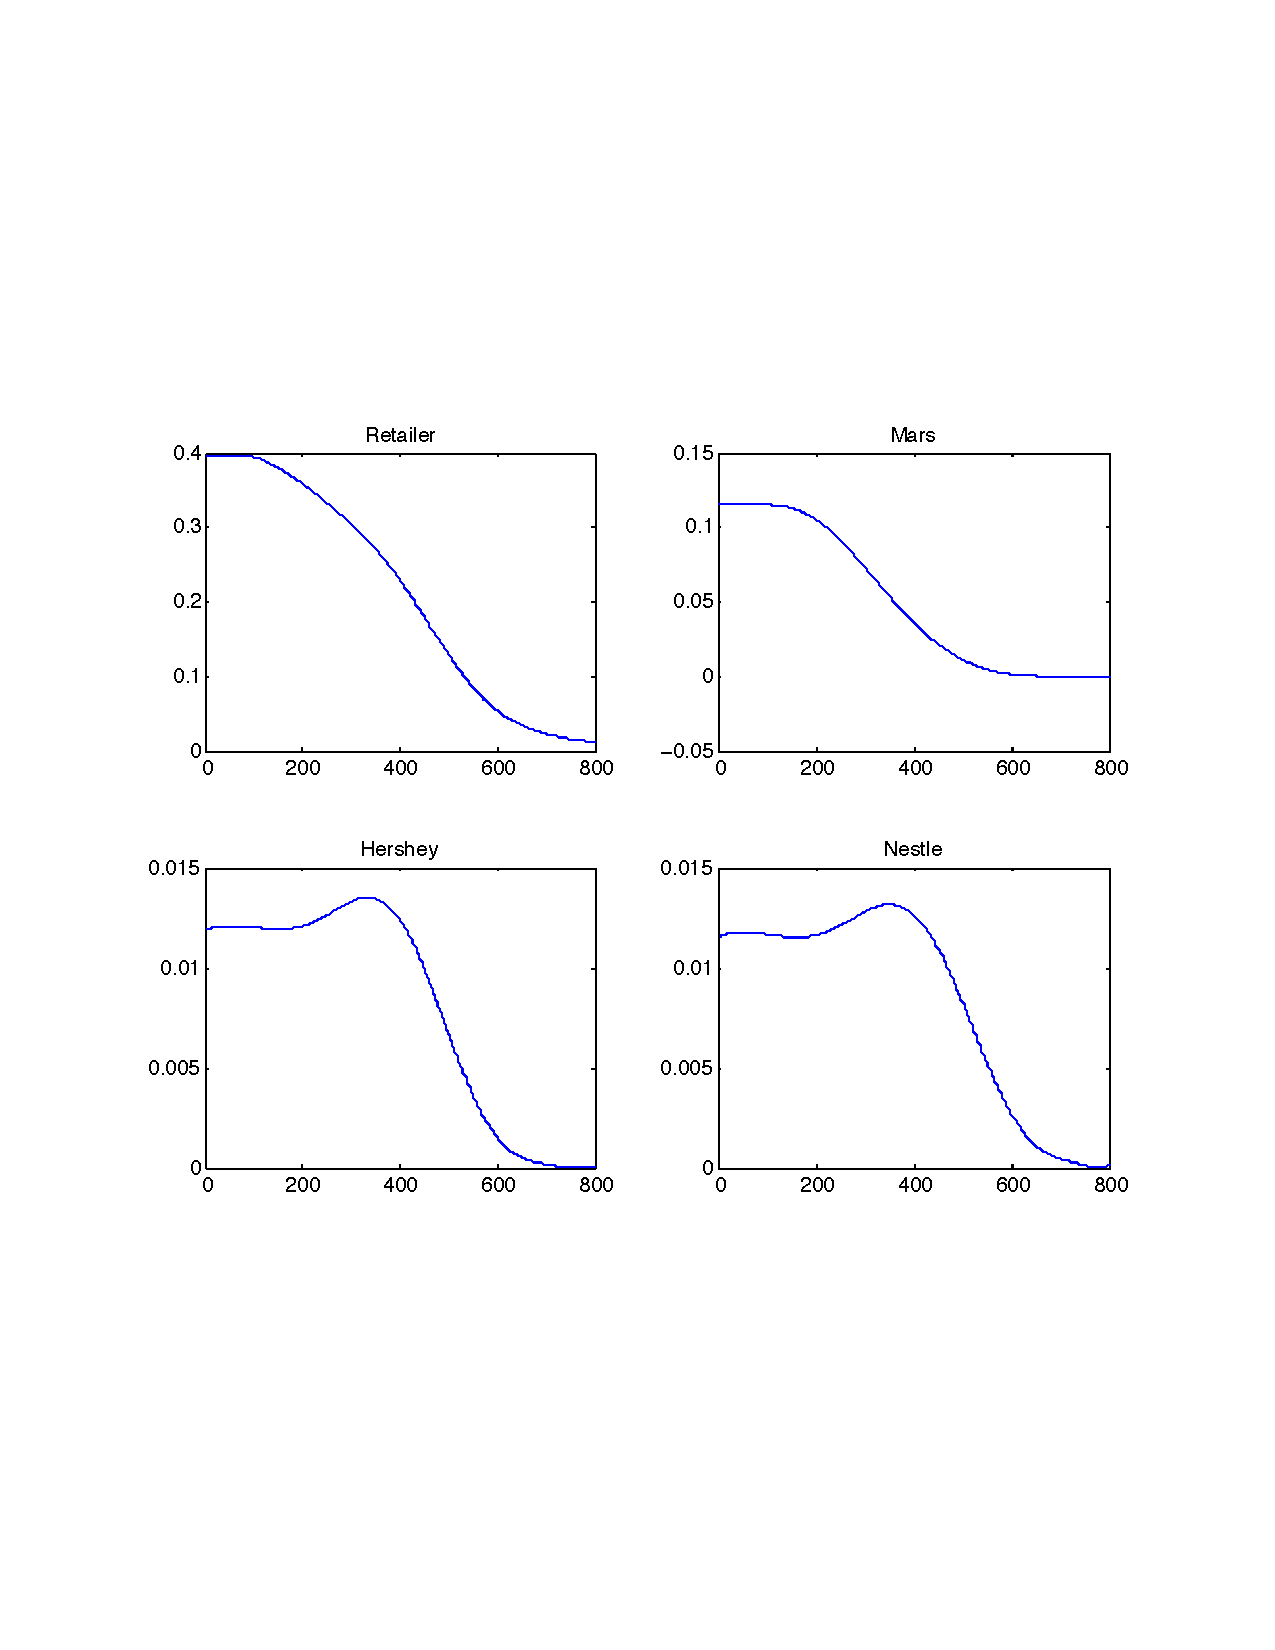
\includegraphics[width=3.3in]{profitsbyfirm.pdf}
\label{fig:profits}
\end{center}
\tiny
Notes: Reports the profits of the retailer, Mars, Hershey and Nestle as a function of the retailer's restocking policy, using the product assortment in which the retailer stocks 3 Musketeers (Mars) and Reese's Peanut Butter Cups (Hershey) in the final two slots. Specifically, the vertical axes report variable profit per consumer for each of the four firms, and the horizontal axes report the number of expected sales between restocking visits.
\end{figure}
\end{frame}


\begin{frame}
\frametitle{Potential Gains from Effort}
\begin{table}[htp]
%\caption{}
\begin{center}
\begin{tabular}{|l | r r r | r r r |}
\hline
&  \multicolumn{3}{c|}{Vertically Integrated}& \multicolumn{3}{c|}{Socially Optimal}\\ 
 & (H,H) & (H,M) & (M,M)  & (H,H) & (H,M) & (M,M) \\ \hline
$\%\Delta(e^{NR}, e^{Opt})$ & 9.89 & 8.61 & 7.95 & 13.69 & 13.11 & 13.26 \\
$\%\Delta(e^{R}, e^{Opt})$ & 7.78 & 6.51 & 6.18 & 11.67 & 11.11 & 11.58 
 \\ \hline
$\Delta \pi^R$ & -83 & -63 & -55 & -163 & -152 & -157 \\
$\Delta \pi^M$ & 195 & 152 & 128 & 251 & 211 & 190 \\
$\Delta PS$ & 76 & 65 & 63 & 39 & 24 & 17 \\
$\Delta CS  (\epsilon=-2)$ & 228 & 210 & 192 & 289 & 290 & 284 \\
$\Delta SS$ & 304 & 275 & 255 & 329 & 313 & 301 \\ \hline
\end{tabular} 
\end{center}
\label{tab:effortnew}
\footnotesize
Notes: Percentage change in policy is calculated as increase required from baseline policy $e^{NR}$ to vertically integrated or socially optimal policy. Social optimum assumes $\alpha$ corresponding to a median own price elasticity of demand of $\epsilon=-2$. For robustness, see Appendix A.4.
\end{table}
\end{frame}





\begin{frame}[label=neteffect]
\frametitle{Net Effect of Efficiency and Foreclosure}
\begin{table}[htp]
%\caption{}
\begin{center}
\begin{tabular}{| l | r | r r r|} 
\hline
&Foreclosure Only&\multicolumn{3}{c|}{Efficiency and Foreclosure}\\
Base:  &$(H,H)$, $e^{R}$& \multicolumn{3}{c|}{ $(H,H)$ and $e^{NR}$} \\ 
to  $(M,M)$ and &$e^R$& $e^{R}$ & $e^{VI}$ & $e^{SOC}$ \\ \hline
$\Delta \pi^R$  & -570& -575 & -626 & -728 \\
$\Delta \pi^M$  & 2,995 & 3,045 & 3,140 & 3,201 \\
$\Delta PS$  & 229 & 267 & 302 & 255 \\
$\Delta CS$ ($\epsilon=-2$) & 150 & 211 & 352 & 444 \\
$\Delta SS$  & 379 & 477 & 654 & 700 \\ \hline
\end{tabular}
\end{center}
\footnotesize
\label{tab:both}
\end{table}
Notes: Transfer at observed rate is \$2,096. Consumer Surplus calibrates $\alpha$ to median own price elasticity of $\epsilon=-2$. Calibration only affects the scale of consumer surplus calculations, not the ranking of various options. 
\hyperlink{more}{\beamerbutton{More}}
\end{frame}

\begin{frame}[label=deviations]
\frametitle{Potential Upstream Deviations}
\footnotesize
\begin{table}[htp]
%\caption{}
\begin{center}
\begin{tabular}{| r | r r r|} 
\hline
\multicolumn{1}{|r|}{Base: } & \multicolumn{3}{c|}{ $(H,H)$ and $e^{NR}$} \\ 
\multicolumn{1}{|r|}{to  $(M,M)$ and} & $e^{R}$ & $e^{VI}$ & $e^{SOC}$ \\ \hline
$\Delta \pi^R$ & -575 & -626 & -728 \\
$\Delta \pi^M$ & 3,045 & 3,140 & 3,201 \\
$\Delta \pi^H$ & -2,173 & -2,173 & -2,173 \\
$\lambda \pi^M$ & 2,096 & 2,111 & 2,121 \\ \hline
$w_h$ to avoid &&&\\
Foreclosure  & 12.83 & 13.54 & 15.35 \\
Reduction in $\lambda$ &&&\\
$(w_h=0.15)$  & 5.27\% & 3.53\% & -0.84\% \\ \hline
\end{tabular}
\end{center}
\label{tab:discount}
\end{table}
\hyperlink{moredeviations}{\beamerbutton{More}}
\end{frame}

\begin{frame}
\frametitle{Linear Pricing vs. AUD (Assortment is (M,M))}
How does the AUD reduce the price of foreclosure? \\ (Compare to linear pricing.)
\begin{table}[h!]
  \begin{center}
%\footnotesize
%  \caption{}
   \label{tab:linearpricing}
    \begin{tabular}{|l|rrr|} 
    \hline 
%          & \multicolumn{3}{|c}{Linear Pricing vs. AUD (Assortment is (M,M))}  \\ 
%          &       &       &       &  \\ \hline
          & $e^{R}$ & $e^{VI}$ & Linear Pricing   \\ \hline
    $\overline{\pi}^M$ & $\in[11912,13101]$ & =13,195 & =0      \\
    $e$ & 259   & 243   & 257    \\
    $\pi^R + \lambda \pi^M$ & 38,182 & 38,146 & 39,103   \\
    $(1-\lambda) \pi^M$ & 11,005 & 11,084 & 10,094   \\
 %   Hershey's Profits & 0     & 0     & 0       \\
%    Nestle Profit & 1,254 & 1,246 & 1,253   \\
%%removed for AER version    Integrated (Mars-Retailer) Profit & 49,187 & 49,230 & 49,197   \\ 
\hline
    PS & 50,441 & 50,476 & 50,450         \\ 
    CS $(\epsilon=-2)$& 24,812 & 24,953 & 24,832         \\ \hline 
   \end{tabular}
   \end{center}
 \tiny
Notes: The optimal wholesale price under linear pricing is estimated to be 41.36 cents per unit.  Hershey is excluded in the (M,M) assortment for all three arrangements, and earns zero profit.  The changes in producer surplus include small changes in Nestle's profits due to the effect of changes in the retailer's choice of restocking policy on the sales of Raisinets. 
\end{table}

\end{frame}

\begin{frame}
\frametitle{Comparison under Alternate Ownership Structures}
\begin{table}[htbp]
  \begin{center}
%    \footnotesize
  \label{tab:merger}
    \begin{tabular}{|l | rrrr|}
\hline
          & No Merger & M-H Merger & M-N Merger & H-N Merger \\
\hline
     AUD Ass. & $e^{VI}(M,M)$ & $e^{VI}(H,M)$ & $e^{VI}(M,M)$ & $e^{VI}(M,M)$ \\
    Alt. Ass. & $e^{NR}(H,H)$ &  $e^{NR}(N,N)$ &  $e^{NR}(H,H)$ &  $e^{NR}(H,H)$ \\
%    Policy & Integrated & Integrated & Integrated & Integrated \\
    \hline
 %   $\Delta$ Retail & 1,497 & 1,579 & 1,753 & 1,497 \\
 %   $\Delta$ Mars & 1,004 & 1,113 & 714   & 1,004 \\
 %   $\Delta$ Bilateral & 2,501 & 2,692 & 2,467 & 2,501 \\
 %   $\Delta$ Competitor & -2,173 & -1,455 & -2,173 & -2,208 \\
 %   $\Delta_r$ + $\Delta_C$ & -676  & 124   & -420  & -711 \\
 %    \hline
 %        $\Delta$ CS & 905   & 2,018 & 884   & 905 \\
 %   $\Delta$ Ind & 293   & 1,236 & 294   & 293 \\
 %   $\Delta$ SS & 1,198   & 3,254 & 1,178   & 1,198 \\
 %    \hline
 %    Price to Avoid Exclusion $c=0$ & 13.30 & n/a   & 8.26  & 13.77 \\
 %   Rebate Reduction $c=0$ & n/a   & 6\%   & n/a   & n/a \\
 %   Rebate Reduction $c=0.15$ & 4\%  & 29\%  & 15\%  & 3\% \\
 
 $\Delta \pi^R$ & -626 & -254 & -621 & -626 \\
$\Delta \pi^M$ & 3,140 & 2,962 & 3,095 & 3,140 \\
$\lambda \pi^M$ & 2,111 & 2,105 & 2,310 & 2,111 \\
$\Delta \pi^{Rival}$ & -2,173 & -1,458 & -2,173 & -2,212 \\ 
\hline
$P^*$ & 13.54 & -11.31 & 9.52 & 13.79 \\
\%$\Delta T^{**}$ & 3.53\% & 43.42\% & 12.67\% & 3.01\% \\
 %   $\Delta \pi^R$ & 1,485 & 1,851 & 1,689 & 1,485 \\
%    $\Delta \pi^M$ & 1,029 & 857   & 785   & 1,029 \\
%    $\Delta \pi^M+\pi^R$ & 2,514 & 2,708 & 2,474 & 2,514 \\
%    $\Delta \pi^{competitor}$ & -2,173 & -1,458 & -2,173 & -2,212 \\
%    $\Delta \pi$ Retailer $+$ Competitor & -688  & 393   & -484  & -727 \\
\hline
%    $\Delta$ CS & 952   & 2,082 & 932   & 952 \\
    $\Delta PS$  & 302   & 1,251 & 302   & 302 \\
    $\Delta CS$ & 444   & 2,473 & 436   & 444 \\
\hline
%    Price to Avoid Exclusion  &              13.54  &  n/a  &                9.52  &              14.05  \\
%    Rebate Reduction $(c=0)$ & n/a   & 18.7\% & n/a   & n/a \\
%    Rebate Reduction $(c=0.15)$ & 3.5\% & 42.3\% & 12.1\% & 2.3\% \\
%    Real Loss to Competitor ($c = 0$) &              2,173  &              1,458  &              2,173  &              2,212  \\
%    Real Loss to Competitor $(c=0.15)$&              1,411  &                 961  &              1,411  &              1,436  \\
%\hline
    \end{tabular}
\end{center}
%\footnotesize
\tiny
Notes: Table compares the welfare impacts of an exclusive Mars stocking policy under alternative ownership structures. This assumes threshold is set at the vertically-integrated level in order to maximize efficiency gains.\\
$^*$Price to avoid foreclosure.
$^{**}$Assumes a marginal cost $c=0.15.$\\
\end{table}
\end{frame}


\begin{frame}
\frametitle{Conclusion}
\begin{itemize}
\item We find both efficiency and foreclosure effects of an AUD.
\item The AUD functions in a way that is analogous to tying.
\item Hershey is foreclosed; the AUD fails to attain the socially-optimal assortment.
\item True efficiency effects of more frequent restocking are small.
\item Rivals are hurt by increased retailer effort.
\item Nevertheless, total profits and consumer welfare are higher compared to a `retailer optimal' outcome without a rebate.
%\item (A Mars-Hershey merger attains the industry-optimal assortment.)
\end{itemize}
\end{frame}


\begin{frame}[label=supplemental]
\frametitle{Theory: Foreclosure}
Start with the following (simple) setup:
\begin{itemize}
\item A retailer $R$ has two remaining places on the shelf.
\item Two manufacturers are selling products: a ``dominant'' firm $M$ and a rival $H$.
\item Retailer can choose three assortments: $a \in \{ (H,H), (H,M), (M,M)\}$.
\item Retail prices are fixed, so that $a$ is only choice.
\item Can order the profits for each agent:
\begin{eqnarray*}
\label{profitorder}
\nonumber \text{Retailer:  } \pi^R(H,H) >& \pi^R(H,M) &> \pi^R(M,M)\\
\nonumber \text{Rival, H:  }\pi^H(H,H) >& \pi^H(H,M) &> \pi^H(M,M)\\
\text{Dominant, M:  }\pi^M(H,H) <& \pi^M(H,M) &<  \pi^M(M,M)
\end{eqnarray*}
\item This closely parallels our empirical exercise.
\end{itemize}
\end{frame}


%\section{Theory}
\begin{frame}
\frametitle{Conditions for Full Foreclosure}
%Outline 3 Sets of 
First, temporarily ignore $(H,M)$
\begin{itemize}
\item Suppose $M$ offers $R$ a transfer $T$ conditioned on foreclosing $H$
\item Define $\Delta \pi^{*}$ as $\pi^*(M,M) - \pi^*(H,H)$ for agent $ ^*$ \\ 
\hspace{0.4in} $\Delta \pi^{R} = \pi^R(M,M) - \pi^R(H,H)$, etc.
\item Three Equilibrium Conditions for Full Foreclosure:
\end{itemize}
\begin{description}
\item[(A1)] $\Delta \pi^R+ T \geq 0$\\
 Incentive Compatible: $T$ induces $R$ to switch (H,M)
\item[(A2)] $\Delta \pi^M - T \geq 0$\\
Individually Rational: $M$ wants to offer T
\item[(A3)] $\Delta \pi^M + \Delta \pi^R + \Delta \pi^H \geq 0$\\
Efficiency: Foreclosure improves industry profits.\\
Or, $-\Delta\pi^H \leq \Delta \pi^M + \Delta \pi^R$ ``Rival can't outbid." 
\end{description}
\end{frame}

\begin{frame}
\frametitle{Conditions for Partial Foreclosure}
Next, temporarily ignore $(M,M)$
\begin{itemize}
\item Define $\Delta_H \pi^{*}$ as $\pi^*(H,M) - \pi^*(H,H)$ for agent $ ^*$ 
\item Consider paying transfer $T_H$ to switch from $(H,H)$ to $(H,M)$
\item Three Equilibrium Conditions for Partial Foreclosure
\end{itemize}
\begin{description}
\item[(B1)] $\Delta_H \pi^R+ T_H \geq 0$
\item[(B2)] $\Delta_H \pi^M - T_H \geq 0$
%\item[(B3)] $\Delta_H \pi^M + \Delta_H \pi^R + \Delta_H \pi^H \geq 0$
\item[(B3)]$-\Delta_H\pi^H \leq \Delta_H \pi^M + \Delta_H \pi^R$
\end{description}
\end{frame}


\begin{frame}
\frametitle{Moving from Partial to Full Foreclosure}
Temporarily Ignore $(H,H)$
%(Considering the change from Partial to Full Foreclosure)
\begin{itemize}
\item Define $\Delta_M \pi^{*}$ as $\pi^*(M,M) - \pi^*(H,M)$ for agent $ ^*$ 
\item Consider paying transfer $T_M$ to switch from $(H,M)$ to $(M,M)$
\item Three Conditions:
\begin{description}
\item[(C1)] $\Delta_M \pi^R+ T_M \geq 0$
\item[(C2)] $\Delta_M \pi^M - T_M \geq 0$\\
\hspace{-0.8in}Either:
\item[(C3)]  $-\Delta_M \pi^H  \leq \Delta_M \pi^M + \Delta_M \pi^R$ \\
Rival can't outbid.\\
\hspace{-0.8in}Or:
\item[(C4)] $-\Delta_M \pi^H  > \Delta_M \pi^M + \Delta_M \pi^R \geq 0$\\
Rival can outbid.
%Rival can outbid
\end{description}
\item C3 and C4 are mutually exclusive. 
%(C3) equivalent (A3), (B3). \\ (C4) applies when $H$'s loss exceeds the net gain of $(R+M)$. 
\end{itemize}
\end{frame}


\begin{frame}
\frametitle{Equilibrium Foreclosure}
\small
%\begin{itemize}
Suppose that (A1)-(C3) hold. 
\begin{itemize}
\item $M$ pays $R$ transfer $T$ to switch from $(H,H) \rightarrow (M,M)$.
\item $(M,M)$ is the equilibrium outcome 
\item By (A3) and (C3), it maximizes industry profits.
\item Foreclosure happens, but it improves welfare. % Caveat: for same p and mc of production across products.
\end{itemize}
\pause
Suppose that (A1-C2)$+$(C4) holds instead.
\begin{itemize}
\item Transfer $T$ is still IC and IR for $R$ and $M$.
\item But losses to $H$ exceed bilateral gains to $R$ and $M$
\item Either $(H,M)$ or $(M,M)$ is the equilibrium outcome.
\item $\Delta_M \pi^M + \Delta_M \pi^R \geq 0$:\\ 
$(M,M)$ maximizes \alert{bilateral surplus} to $R$ and $M$.
\item $-\Delta_M \pi^H  > \Delta_M \pi^M + \Delta_M \pi^R$: \\
$(H,M)$ maximizes \alert{industry surplus}.
\end{itemize}
%\end{itemize}
\end{frame}

\begin{frame}
\frametitle{Chicago Critique}

If $M$ can condition the transfer $T$ on achieving $(M,M)$, \\
then $(M,M)$ is the equilibrium outcome.
%\pause
\begin{itemize}
\item Full foreclosure of $H$ is \alert{not socially optimal}.
\item But it happens anyway.  
\item Partial foreclosure {\it is} optimal.
\item By conditioning $T$ on the $(M,M)$ outcome, \\ $M$ effectively ties the products.
\end{itemize}
Back to \hyperlink{intuition}{\beamerbutton{Intuition}}.
\end{frame}

\begin{frame}[label=param_supp]
\frametitle{Parameters of Consumer Choice Model}
\scriptsize
%\vspace{-0.25in}
%\caption {Parametric Model Estimates}
\label{parameters}
\begin{center}
\begin{tabular}{ | l  | r r | }%r r | }
\hline
Random Coefficients:&\multicolumn{2}{c|}{Parameter Estimates}\\%& \multicolumn{2}{c|}{Nested Logit}\\
\hline \hline
$\sigma_{Salt}$&0.506&0.458\\%& & \\
&[.006]&[.010]\\%& & \\
$\sigma_{Sugar}$&0.673&0.645\\%& & \\
&[.005]&[.012]\\%& & \\
$\sigma_{Peanut}$&1.263&1.640\\%& & \\
&[.037]&[.028]\\%& & \\
%$\lambda_{Chocolate}$& & &0.828&0.810\\
%& & &[.003]&[.005]\\
%$\lambda_{Candy Non-Choc}$& & &0.908&0.909\\
%& & &[.007]&[.009]\\
%$\lambda_{Cookie/Pastry}$& & &0.845&0.866\\
%& & &[.004]&[.006]\\
%$\lambda_{Other}$& & &0.883&0.894\\
%& & &[.005]&[.006]\\
%$\lambda_{Salty Snack}$& & &0.720&0.696\\
%& & &[.003]&[.004]\\
\hline
%\# Nonlinear Params&3&3&5&5\\
%Product FE&73&73&73&73\\
\# Fixed Effects $\xi_t$&15,256&2,710\\%&15,256&2,710\\
%Total Parameters&15332&2786&15334&2788\\
\hline
LL&-4,372,750&-4,411,184\\%&-4372147&-4410649\\
%Total Sales&2960315&2960315\\%&2960315&2960315\\
BIC&8,973,960&8,863,881\\%&8972783&8862840\\
AIC&8,776,165&8,827,939\\%&8774962&8826873\\
\hline
\end{tabular}
\end{center}
\tiny
Both specifications include 73 product fixed effects.  Total sales are 2,960,315. 
\hyperlink{param_main}{\beamerbutton{Back}}
\end{frame}

\begin{frame}[label=supplemental1]
\frametitle{Details, Re-stocking Model}
Similar to Rust (1987): estimate the retailer's optimal wait until the next re-stocking visit (as a function of expected sales).
\vfill
\begin{itemize}
\item Start from a `full machine' with assortment $a$.
%\item To obtain $\pi(x)$, e
\item Estimate the consumer choice model; specify an arrival process of `likely consumers' $f(x' | x)$.
\begin{itemize}
\item Use arrival rate at `higher than average volume' machines.% to calibrate consumer arrival process.
\end{itemize}
\item Simulate arrivals; after each consumer choice, update product-level inventories and adjust set of available products.
\item Average over 100,000 simulated chains to construct expected profit after $x$ consumers have arrived.
\item Fit a smooth Chebyshev polynomial; use this to approximate profits of each agent.
%construct expected profit after $x$ `likely consumers.'
%\item Convert expected profits to a function of `likely consumers' 
%\item In theory, we should be able to estimate $FC$, but our retailer sets a level of service that is too high to rationalize with any optimal stocking behavior.
\end{itemize}
\vfill
\hyperlink{main}{\beamerbutton{Back}}
\end{frame}

%\begin{frame}
%\frametitle{Key Welfare Questions}
%%Given demand parameters $\hat{\theta}$:
%%\begin{enumerate}
%%\item Forward Simulate sales for a machine with choice set $a$ from full to completely empty as a function of $x$.
%%\item Pick a policy $e = x^{*}$.
%%\item Given $(\tilde{w_m},w_n)$ we can compute $\pi_R(a,e)$, $\pi_M(a,e)$, $\pi_H(a,e)$ at ANY $(a,e)$.
%%\end{enumerate}
%Vary $(\tilde{w}_m,w_n)$ and analyze:
%\begin{itemize}
%\item Does the observed rebate program lead to exclusion?
%\item Is Mars willing to pay for exclusion at observed rebate level?
%\item Could Hershey set $w_h = mc_h$ to avoid exclusion?
%\item Does a Mars-exclusive assortment maximize industry profits? (Chicago Critique)
%\end{itemize}

%\end{frame}

\begin{frame}[label=supplemental2]
\frametitle{Simulating the Payoff of a Re-stocking policy}
\vfill
\begin{itemize}
\item For R, with assortment $a$ and effort policy $e$, the net present value of the long-run average profit of a typical machine is: 
\begin{eqnarray}
\label{retail_payoffs}
\pi^R(a,e) = \Gamma(\tilde{P}(e)) \cdot(I - \beta \tilde{P}(e))^{-1} \cdot \hat{u}^R(x,a).
\end{eqnarray}
\item The ergodic distribution of $x$ as a function of the restocking policy is given by the solution $\Gamma$ to $\Gamma= \Gamma \tilde{P}(e). $ 
%\item $(I - \beta \tilde{P}(e))^{-1}$ represents the present discounted value of a stream of payments. 
\item  Both $\Gamma(\tilde{P}(e))$ and $(I - \beta \tilde{P}(e))^{-1}$ depend on effort only through the post-decision transition matrix $\tilde{P}(e)$). 
\item $\hat{u}^R(x,a)$ is the simulated cumulative payoff function, which depends only on $a$ (and the state variable $x$). 
\item To evaluate profits for different agents, replace $\hat{u}^R(x,a)$ with $\hat{u}^M(x,a)$; evaluate at the same policy $e$.
\end{itemize}
\vfill
\hyperlink{main}{\beamerbutton{Back}}
\end{frame}


\begin{frame}[label=moredeviations]
\frametitle{Potential Upstream Deviations}
\footnotesize
\begin{table}[htp]
%\caption{}
\begin{center}
\begin{tabular}{| r | r r r | r r r|} 
\hline
\multicolumn{1}{|r|}{Base: }& \multicolumn{3}{c|}{$(H,M)$ and $e^{NR}$ }  & \multicolumn{3}{c|}{ $(H,H)$ and $e^{NR}$} \\ 
\multicolumn{1}{|r|}{to  $(M,M)$ and}& $e^{R}$ & $e^{VI}$ & $e^{SOC}$ & $e^{R}$ & $e^{VI}$ & $e^{SOC}$ \\ \hline
$\Delta \pi^R$ & -312 & -364 & -466 & -575 & -626 & -728 \\
$\Delta \pi^M$ & 1,382 & 1,476 & 1,538 & 3,045 & 3,140 & 3,201 \\
$\Delta \pi^H$ & -1,302 & -1,302 & -1,302 & -2,173 & -2,173 & -2,173 \\
$\lambda \pi^M$ & 2,096 & 2,111 & 2,120& 2,096 & 2,111 & 2,121 \\ \hline
$w_h$ to avoid &&&&&&\\
Foreclosure & -15.83 & -14.61 & -11.59 & 12.83 & 13.54 & 15.35 \\
Reduction in $\lambda$ &&&&&&\\
$(w_h=0.15)$ & 44.79\% & 42.72\% & 38.18\% & 5.27\% & 3.53\% & -0.84\% \\ \hline
\end{tabular}
\end{center}
\label{tab:discount}
\end{table}
\hyperlink{deviations}{\beamerbutton{Less}}
\end{frame}


\end{document}


\begin{frame}
\frametitle{}
\end{frame}





\begin{frame}
\frametitle{}
\end{frame}

\begin{frame}
\frametitle{}
\end{frame}

\begin{frame}
\frametitle{}
\end{frame}





\begin{frame}
\frametitle{}
\end{frame}

\begin{frame}
\frametitle{}
\end{frame}

\begin{frame}
\frametitle{}
\end{frame}





\begin{frame}
\frametitle{}
\end{frame}

\begin{frame}
\frametitle{}
\end{frame}

\begin{frame}
\frametitle{}
\end{frame}


\begin{frame}
\frametitle{}

\end{frame}


\begin{frame}
\frametitle{}
\end{frame}

\begin{frame}
\frametitle{}
\end{frame}

\begin{frame}
\frametitle{}
\end{frame}






\begin{frame}
\frametitle{}
\end{frame}

\begin{frame}
\frametitle{}
\end{frame}

\begin{frame}
\frametitle{}
\end{frame}



\subsection{Numerical Example (Retailer Assortment)}

\begin{frame}
  \frametitle{Toy Model: Agents}
\begin{itemize}\footnotesize
\item Two upstream firms (M and H).  
	\begin{itemize}\scriptsize
	\item Firm M sells two products: 1 and 3.
	\item Firm H sells one product: 2.
	\item Production costs of M and H are zero.
	\item Firm M offers an AUD.
	\item M and H sell to the downstream firm (R) at wholesale prices $w_M$ and $w_H$. (Thus, firm M sells products 1 and 3 at the same wholesale price.)
	\end{itemize}
\item One downstream firm R
	\begin{itemize}\scriptsize
	\item Charges a single price $p$ for all products
	\item Faces the same capacity for all products.
	\end{itemize}
\item Consumers:
	\begin{itemize}\scriptsize
	\item Each consumer has a ranking over two possible products, \\ including an outside good (0).
	\item No consumer ranks the outside good first.
	\item Random arrival of 100 consumers.
	\end{itemize}
\end{itemize}
\end{frame}


\begin{frame}
  \frametitle{Toy Model:  AUD and Choice Variables}
\footnotesize
Downstream firm R's cost is:
\begin{equation}
C(q_M,q_H) = w_M \cdot q_M - \mathbf{1}[q_M > \overline{q_M}] \cdot  \Delta \cdot q_M + w_H \cdot q_H
\end{equation}

\begin{itemize}\footnotesize
\item Upstream firm M chooses:
	\begin{itemize}\scriptsize
	\item Wholesale price $w_M$.
	\item Size of discount, $\Delta$.
	\item Quantity threshold $\overline{q_M}$.
	\end{itemize}
\item Upstream firm H chooses $w_H$.
\item Downstream firm R chooses:
	\begin{itemize}\scriptsize
	\item Two products to stock ([1,2], [1,3], or [2,3]), denoted as availability $a$.
	\end{itemize}
\item Consumers:
	\begin{itemize}\scriptsize
	\item Consumers choose 1 product from the set of 2 products offered by R.
	\item If neither of her first two choices are available, she leaves the market.
	\end{itemize}
\end{itemize}
\end{frame}


\begin{frame}
  \frametitle{Toy Model:  Simulation}
\footnotesize
The model:
\begin{itemize}
\item Random arrival of 100 consumers
\item Assign product rankings so that, in the absence of any constraints, $q_1 \geq q_2 \geq q_3$.
\item Under the assumed demand patterns, retailer always stocks product 1, and product 2 is a `closer substitute' to product 1 than is product 3.
\item $p$ = \$1, $w_M = \$0.40$, $w_H = \$0.20$, $\Delta = \$0.15$, $\overline{q} = 65$, 
\end{itemize}
Simulate the model 100,000 times to account for differences in outcomes based on the random ordering of consumers.\\

\end{frame}


\begin{frame}
  \frametitle{Toy Model:  Results (Vary Capacity)}
\begin{table}[htdp]\tiny
\begin{center}
\begin{tabular}{|l|rr|}
\hline
Threshold $\overline{q} = 65$   &Capacity = 45 & Capacity = 65\\
\hline
\bf{Market:}&&\\
Total Sales([1,2]) $>$ Total Sales([1,3])&66.72\%&24.16\%\\
Total Sales([1,2]) $<$ Total Sales([1,3])&26.49\%&66.59\%\\
Total Sales([1,2]) $=$ Total Sales([1,3])&6.79\%&9.25\%\\
Mean(Sales([1,2])-Sales([1,3]))&2.92 &-2.00 \\
\hspace{0.3in} as percent of sales&3.36\%&-2.17\%\\
\bf{Retailer:}&&\\
Retailer prefers [1,2]&25.80\%& 0.61\%\\
Retailer prefers [1,3], No Rebate &$0.33\%$ &$0.69\%$\\
Retailer prefers [1,3]& 74.20\%&99.39\%\\
Mean Retailer profit([1,2])&60.41&63.21\\
Mean Retailer profit([1,3]), No Rebate&$50.36$&$56.68$\\
Mean Retailer profit([1,3])&62.88&70.85\\
\bf{Firm M:}&&\\
Firm M prefers [1,2]&0.19\%&13.78\%\\
Firm M prefers [1,3]&99.55\%&85.43\%\\
Mean Firm M profit under [1,2]&17.98& 21.52\\
Mean Firm M profit under [1,3]&20.96& 23.62 \\
Firm M pays rebate under [1,2]&0\%&0\%\\
Firm M pays rebate under [1,3]&100\%&100\%\\
\bf{Firm H:}&&\\
Mean Firm H profits under [1,2]&8.36&7.73\\
\hline 
\end{tabular}
%\caption{Results from varying capacity in toy model}
\label{toy_model}
\end{center}
\end{table}
\end{frame}


\begin{frame}
  \frametitle{Toy Model:  Comments}
\footnotesize
\begin{itemize}
\item In the absence of the AUD, R will not stock M's products exclusively.
\item The AUD induces exclusivity, but whether exclusivity is efficient (i.e., whether it maximizes industry profits) depends on capacity.
\item Firm M benefits from the AUD (paying the rebate is rational), and firm H is harmed.
\item More generally, we can think of capacity standing in for retailer effort.  (e.g., re-stocking small shelves more frequently)
\end{itemize}

\end{frame}


\begin{frame}
\frametitle{Profits after Mars-Nestle Merger}
\tiny
\begin{table}[htbp]
  \centering
%  \footnotesize
 % \caption{Profits after Mars-Nestle Merger}
    \begin{tabular}{l | rrrrrrrr}
        \hline
\multicolumn{2}{c}{\textbf{Policy}} & \textbf{Retail} & \textbf{Rebate} & \textbf{Mars/} & \textbf{Hershey} & \textbf{Integrated} & \textbf{Industry} & \textbf{Consumer} \\
\multicolumn{2}{c}{\textbf{ }}  & \textbf{(No Reb.)} &&\textbf{Nestle}& & & & \\
\hline
\multicolumn{9}{c}{Reeses PB Cup(H), 3 Musketeers(M)}             \\
\hline
Retailer & 267   & 36,119 &       & 13,302 & 1,305 & 49,421 & 50,726 & 63,371 \\
\textbf{Rebate} & 263   & 36,117 &       & 13,325 & 1,302 & 49,442 & \textbf{50,744} & \textbf{63,425} \\
\textbf{Integrated} & 247   & 36,071 &       & 13,406 & 1,293 & 49,477 & \textbf{50,770} & \textbf{63,571} \\
Industry & 249   & 36,080 &       & 13,397 & 1,294 & 49,477 & 50,771 & 63,559 \\
\hline
\multicolumn{9}{c}{Reeses PB Cup(H), Payday(H)}                \\
\hline
\textbf{Retailer} & \textbf{263} & \textbf{36,384} & \textbf{} & \textbf{11,659} & \textbf{2,173} & \textbf{48,044} & \textbf{50,216} & \textbf{62,600} \\
Rebate & 258   & 36,381 &       & 11,693 & 2,168 & 48,074 & 50,242 & 62,663 \\
Integrated & 241   & 36,326 &       & 11,796 & 2,152 & 48,122 & 50,274 & 62,795 \\
Industry & 243   & 36,336 &       & 11,785 & 2,154 & 48,121 & 50,276 & 62,787 \\
\hline
\multicolumn{9}{c}{3 Musketeers(M), Milkyway(M)}                    \\
\hline
Retailer & 264   & 35,822 & 2,343 & 14,643 & 0     & 50,465 & 50,465 & 63,052 \\
\textbf{Rebate} & \textbf{261} & \textbf{35,821} & \textbf{2,345} & \textbf{14,658} & \textbf{0} & \textbf{50,479} & \textbf{50,479} & \textbf{63,092} \\
\textbf{Integrated} & \textbf{246} & \textbf{35,781} & \textbf{2,356} & \textbf{14,729} & \textbf{0} & \textbf{50,510} & \textbf{50,510} & \textbf{63,231} \\
Industry & 246   & 35,781 & 2,356 & 14,729 & 0     & 50,510 & 50,510 & 63,231 \\
%\hline
%\multicolumn{9}{c}{Butterfinger (N), Crunch (N)}              \\
%\hline
%Retailer & 256   & 35,908 & 2,182 & 13,633 & 0     & 49,541 & 49,541 & 61,696 \\
%Rebate & 252   & 35,906 & 2,185 & 13,658 & 0     & 49,564 & 49,564 & 61,743 \\
%Integrated & 236   & 35,856 & 2,200 & 13,747 & 0     & 49,603 & 49,603 & 61,853 \\
%Industry & 236   & 35,856 & 2,200 & 13,747 & 0     & 49,603 & 49,603 & 61,853 \\
    \end{tabular}%
  \label{mnmerger}%
\end{table}

\end{frame}

\begin{frame}
\frametitle{Profits after Hershey-Nestle Merger}
\tiny
\begin{table}[htbp]
  \centering
%  \footnotesize
%  \caption{Profits after Hershey-Nestle Merger}
% Table generated by Excel2LaTeX from sheet '100k Draws'
\begin{tabular}{l | rrrrrrrr}
        \hline
\multicolumn{2}{c}{\textbf{Policy}} & \textbf{Retail} & \textbf{Rebate} & \textbf{Mars} & \textbf{Hershey/} & \textbf{Integrated} & \textbf{Industry} & \textbf{Consumer} \\
\multicolumn{2}{c}{\textbf{ }}  & \textbf{(No Reb.)} && &\textbf{Nestle}& & & \\
%      & \textbf{Policy} & \textbf{Retail (NR)} & \textbf{Rebate} & \textbf{Mars} & \textbf{Hershey/Nestle} & \textbf{Integrated} & \textbf{Industry} & \textbf{Consumer} \\
            \hline
      & \multicolumn{8}{c}{Reeses PB Cup(H), 3 Musketeers}      \\
            \hline
Retailer & 267   & 36,398 &       & 11,763 & 2,565 & 48,161 & 50,726 & 63,371 \\
\textbf{Rebate} & 263   & 36,395 &       & 11,789 & 2,560 & 48,184 & \textbf{50,744} & \textbf{63,425} \\
\textbf{Integrated} & 246   & 36,342 &       & 11,885 & 2,542 & 48,227 & \textbf{50,769} & \textbf{63,576} \\
Industry & 249   & 36,356 &       & 11,870 & 2,545 & 48,226 & 50,771 & 63,559 \\
      \hline
      & \multicolumn{8}{c}{Reeses PB Cup(H), Payday(H)}        \\
      \hline
\textbf{Retailer} & \textbf{263} & \textbf{36,668} & \textbf{} & \textbf{10,091} & \textbf{3,457} & \textbf{46,759} & \textbf{50,216} & \textbf{62,600} \\
Rebate & 258   & 36,665 &       & 10,128 & 3,450 & 46,793 & 50,242 & 62,663 \\
Integrated & 239   & 36,596 &       & 10,253 & 3,422 & 46,849 & 50,272 & 62,801 \\
Industry & 243   & 36,618 &       & 10,229 & 3,428 & 46,848 & 50,276 & 62,787 \\
\hline
      & \multicolumn{8}{c}{3 Musketeers(M), Milkyway(M)}             \\
      \hline
Retailer & 265   & 36,101 & 2,096 & 13,100 & 1,259 & 49,201 & 50,460 & 63,038 \\
\textbf{Rebate} & \textbf{261} & \textbf{36,099} & \textbf{2,100} & \textbf{13,123} & \textbf{1,257} & \textbf{49,222} & \textbf{50,479} & \textbf{63,092} \\
\textbf{Integrated} & \textbf{245} & \textbf{36,052} & \textbf{2,113} & \textbf{13,208} & \textbf{1,249} & \textbf{49,260} & \textbf{50,509} & \textbf{63,236} \\
Industry & 246   & 36,057 & 2,112 & 13,203 & 1,250 & 49,260 & 50,510 & 63,231 \\
\end{tabular}
  \label{hnmerger}%
\end{table}

\end{frame}

